% Terms and Definitions
%TODO maybe move stuff from chapter 1 in this chapter
\chapter{Metrics and Measurement Methods}

[tbd]


[Last chapter]



[This chapter]

% In this chapter, I will cover measurement methods and discuss common performance metrics
% - This chapter should cover all relevant terms and definitions within web performance measurement
% How terms can be structured / taxonomy
% Ambiguity of definitions




[Relevance of this chapter for research question]





[Next chapter]





[Outline of this chapter]

%- Technical Background
%	   - Network
%	   - Front End: Navigation and CRP

%- Measuring Methods	

%- Metrics





% ---------------------------------------------------------------------------------------------------
% ---------------------------------------------------------------------------------------------------


\section{Technical Background of the Website Loading Process}


% [Introduction]

In order to understand web performance metrics and the methods to measure them, it is crucial to have a basic understanding of the technical aspect of the loading of a website into the browser.
This process includes establishing a connection between a client and a server, which will be discussed in section X, and the task of the browser to transform the received data from the server into a readable ready-to-use website, which will be discussed in section X.
%Always with performance in mind.


% [3 Entities: FE, BE, Network]

It is possible to divide the website loading process into three entities.
In his code talk 2016, Witt identifies three main areas of the website loading process: The Front End, the Back End, and the Network.  % cite 2016 Witt or just say this ??
The Front End is everything the user sees on the screen, client, UI, browser, sends requests to a back end, etc.
The Back End is the logic, server, also data base, handles requests and sends responses to a front end
Network is what connects clients and servers, FE and BE, infrastructure element composed of routers, cables, wireless connections etc.

The main steps can be divided into networking, that is, establishing a connection with DNS etc., backend processing, e.g. data base queries etc., and the rendering in the front end, as seen in image X.
The last part of this process is when browser receives finally the HTML / Document. 
How the browser transfers the HTML into an interactive website is part of the next section.



\begin{figure}[h!]
\begin{center}
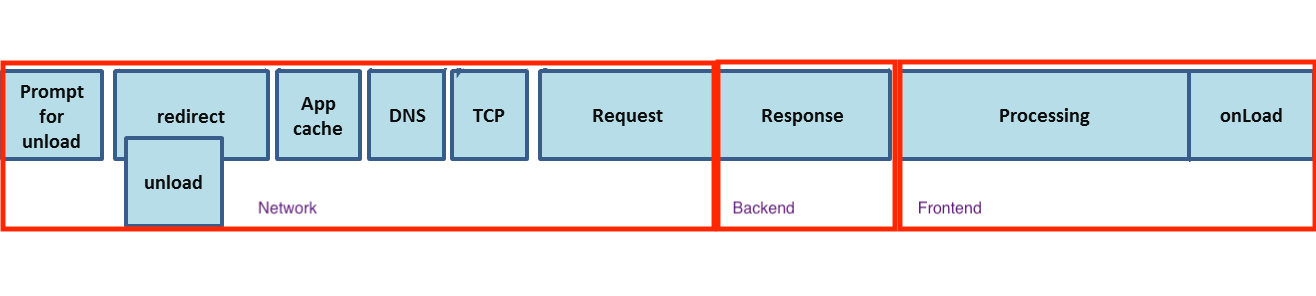
\includegraphics[width=0.8\textwidth]{timing_overview_blanco2.png}
\caption{Timing Overview}
\label{img:timing_overview}
\end{center}
\end{figure}
%TODO change image: make it clean


- BE is not discussed (server time, data base, etc.)
- Section X is about Network
- Section X is about Front end: how browser works, crp, 
- How to optimise websites is not part of this thesis




% [Performance]

Focus and perspective is performance, like in overall thesis.
Also when explaining the technical background, I will keep the aspect of performance in mind.

Once I discussed the processes in the network and the front end, I will move on to the question of how to measure the performance of those processes, and which metrics are available to quantify the performance.


%TODO should I talk about metrics already in this section ?


% --------------------------------------------------------------------------------------------
% --------------------------------------------------------------------------------------------


\subsection{The Website Loading Process in the Network}

[tbd]

The network is... Starting from hardware, ISP, routers, switches etc and the cables connecting them.
But also communication protocols such as the Internet protocol suite.

Regarding performance, latency and bandwidth come into mind, and we will see that latency has a bigger impact on performance than bandwidth in section X.

After discussing this issue, i will continue by describing the process or navigation steps which happen once the user enters a URL into the browser, up until he sees pixels on his screen and can use the website.


% --------------------------------------------------------------------------------------------


\subsubsection{Latency and Bandwidth}

There are two important attributes when discussing network performance: Latency and Bandwidth.
The important thing to say here is that Latency is bottleneck for performance, and not bandwidth.


% [Bandwidth]

Bandwidth is the "maximum throughput of a logical or physical communication path". %cite 2013 Grigorik
In other words, bandwidth describes the amount of data which can be sent in parallel from one node in a network to another. 
Physical communication paths are most likely cables such as metal wires or fiber-optic cables, where fiber-optic cables have less signal loss, and lower lifetime maintenance costs.
With methods such as wavelength-division multiplexing (WDM), it is possible to transmit up to 70 Tbit/s over a fiber-optic connection.  %cite 2013 Grigorik
This high technology stuff is only used in the backbone infrastructure, e.g. for connecting Europe with America.
For the end user, bandwidth is much lower, and the average was in late 2015 just 5.1 Mbps %cite 2013 Grigorik
A high bandwidth is useful for bulk or large data transfer such as streaming of video or audio.
But for loading a website,or any browser activity that depends on many requests that fetch data from many different locations around the globe, the performance bottleneck is latency. % cite 2013 Grigorik


% [Latency]

Latency is "the time from the source sending a packet to the destination receiving it".  % cite 2013 Grigorik
Latency is measured in seconds and can be the time spent for one-way, or more common, how long it takes for the transmitted data package for the round-trip time (RTT), from source to destination and back.
In other words, latency "describes the amount of delay on a network or Internet connection". % cite https://developer.mozilla.org/en-US/docs/Web/Performance/Understanding_latency
For the very first request when establishing a connection, latency is longer due to protocols such as DNS lookup, TCP and TLS handshakes.
Those will be discussed in section X. % cite https://developer.mozilla.org/en-US/docs/Web/Performance/Understanding_latency


% [Experiment]

To get an idea about how the two aspects, bandwidth and latency, impact web performance,  Mike Belshe launched a study. % cite https://docs.google.com/a/chromium.org/viewer?a=v&pid=sites&srcid=Y2hyb21pdW0ub3JnfGRldnxneDoxMzcyOWI1N2I4YzI3NzE2
Once setup has a fixed latency and bandwidth is variable, and vice versa.
He and compared the performance of the two experiments using the Page Load Time metric. (cf. X for this metric)


\begin{figure}[h!]
\begin{center}
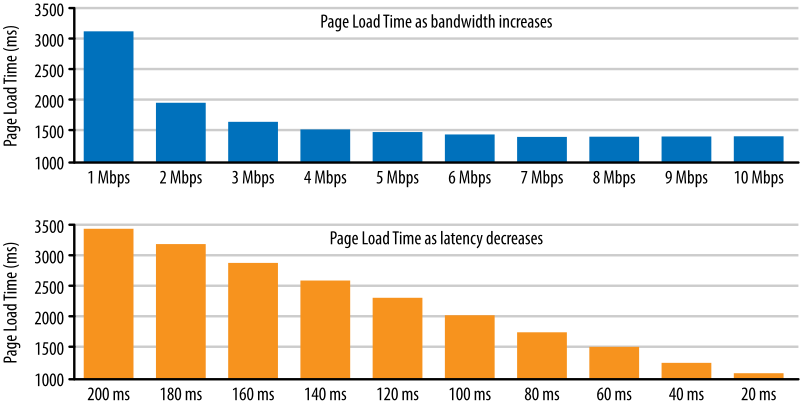
\includegraphics[width=0.8\textwidth]{latency.png}
\caption{Latency vs Bandwidth}
\label{img:latency}
\end{center}
\end{figure}


We can see that the impact of bandwidth is trivial: if the available bandwidth is doubled, e.g. from 5 to 10 Mbps, there is no change in performance load time.
For Latency on the other hand, the picture is different: If the latency can be decreased by half, e.g. from 120 ms to 60 ms, the page load time also sinkt um die hälfte.
Or as Belshe states it, "[reducing] cross-atlantic RTTs from 150ms to 100ms [...] would have a larger effect on the speed of the internet than increasing a user's bandwidth from 3.9Mbps to 10Mbps or even 1Gbps." % cite https://docs.google.com/a/chromium.org/viewer?a=v&pid=sites&srcid=Y2hyb21pdW0ub3JnfGRldnxneDoxMzcyOWI1N2I4YzI3NzE2

This observations can be explained with the many short, small connections and requests are made when browsing websites and the contrary underlying structure of the communication protocols, which are "optimized for long-lived connections and bulk data transfers. " %cite 2013 Grigorik ch 10
But just simply decreasing the latency is not straightforward: The speed of data transfer is already at a 2/3 of light, but the physical constraint is the limiting factor, e.g. there is a minimum distance between London and New York which can not be further "optimized". % cite 2013 Grigorik Ch 1


% [Mobile]

Another aspect of latency is that for wireless connections and therefore mobile devices, latency is even higher, "making networking optimization a critical priority for the mobile web." % cite 2013 Grigork Ch 1
This is due to the infrastructure of mobile nets, latency is high for mobile users. cf.  Why are mobile latencies so high? in Grigorik % cite https://www.igvita.com/slides/2013/fluent-perfcourse.pdf


% [Transition]

As latency is a important factor, what happens on the front end is still important.
And again for this thesis metrics measuring performance in the front end are the focus.

Before i will discuss what happens in the browser once the website data arrived, i will briefly describe the preceding steps of establishing a connection between the browser (client) and the server, which can be considered to be still a part of the network.




%TODO add this ?
% Use other techniques such as CDNs, caching, pre-fetching, etc % 2013 Grigorik
% CDN: Help against this issue. Put stuff close to client % 2013 Grigorik
% Some direct implications for performance measurement ?
% Understanding Latency https://developer.mozilla.org/en-US/docs/Web/Performance/Understanding_latency
% Network throttling: Emulate download speed, upload speed, and minimum latency



% --------------------------------------------------------------------------------------------


\subsubsection{Network Navigation Steps}

[tbd]

I will explain briefly the main navigation steps: It begins when the user is submitting a URL in the browser and ends when he received website data.

"To start, it is important to recognize that every HTTP request is composed of a number of separate stages (Figure 10-3): DNS resolution, TCP connection handshake, TLS negotiation (if required), dispatch of the HTTP request, followed by content download." % cite Grigorik 2013


%TODO add this ?
% Understanding Latency https://developer.mozilla.org/en-US/docs/Web/Performance/Understanding_latency
%Network Timings:
%- Blocked: When a request is in queue
%- Blocking happens when there are too many simultaneous connections to single server over HTTP



% ----------------------------------


\paragraph{DNS Lookup}

When the requested resource can not be loaded from the browsers cache, the first step to establish a connection is a DNS Lookup (or DNS Resolution).

This step is about translate URL to IP address.
Must be done for each unknown URL, e.g. when linked images within a website are from different server, for each unique URL DNS Lookup has to be done.
The mapping of URL to IP can be cached by browser, which makes repeated views faster. % cite https://developer.mozilla.org/en-US/docs/Web/Performance/How_browsers_work

Avg. time is 20 and 120 ms % https://www.keycdn.com/support/reduce-dns-lookups

%Metric?
%Can be considered a performance metric, see section X.


% ----------------------------------


\paragraph{TCP Handshake}

Once a connection between a client and a server is established, the TCP 3-way-Handshake comes into play.

The goal of TCP is to establish a reliable connection within an unreliable network.
TCP  "guaranteed that all bytes sent will be identical with bytes received and that they will arrive in the same order to the client. " %cite 2013 Grigorik
Regarding performance, the handshake adds two more round trips, which is bad for performance as we have seen because of latency.

Many algorithms and techniques to get optimal data transfer and also avoid congestion are existing, such as Slow-Start.
Slow-Start is an algorithm that determines the maximum bandwidth that can be used by gradually increasing the amount of data sent.
Slow start prevents that the full capacity of the network is being used from the beginning, which in performance terms adds again more round trips and latency. %cite 2013 Grigorik

For a detailed discussion cf "Building Blocks of TCP" in 2013 Grigorik % cite https://hpbn.co/building-blocks-of-tcp/

%TODO once i know which metric add it here ?
%A performance metric reflecting the time spent for establishing a TCP connection is X, see section X.




% ----------------------------------


\paragraph{TLS Negotiation}

TLS is another protocol which has the goal to establish a secure connection in terms of data encryption.
Data transmitted over the network has to be encrypted so that aussenstehende can not read or manipulate the data.
For encryption,  a cipher to be used needs to be established, which will be shared between client and server during the TLS Negotiation. % cite https://developer.mozilla.org/en-US/docs/Web/Performance/How_browsers_work

TLS again adds more round trips which is bad for performance.

for a detailed discussion see Transport Layer Security (TLS) in 2013 Grigorik % https://hpbn.co/transport-layer-security-tls/

%TODO once i know which metric add it here?
%A performance metric reflecting the time spent for a TLS negotiating is blabla in section X.


% ----------------------------------


\paragraph{HTTP Request and Response}

Now that a secure connection is established, the client fetches the first resources via HTTP GET request.
Most often, the server will respond by sending back the index.html file, which then can be used by the browser to build the website. % cite https://developer.mozilla.org/en-US/docs/Web/Performance/How_browsers_work

The time when this first response containing the first byte for building the web site is reflected in the metric TTFB which is discussed in section X.


% [Connection vs Request]

Usually, many more resources are requested by the browser to complete the build of the web site.
As of today, the median value is about 70 requests per web site. % footnote https://httparchive.org/reports/state-of-the-web#reqTotal

A request is not the same as a connection.
Once the connection is established via the above described procedures such as DNS lookup, TCP and TLS handshakes, multiple requests can be transmitted over the same connection.
Usually, the number of requests is much higher than the number of connections to load a website, as the browser persist connections, keep them open for multiple requests.
Median connections for a web site today is about 13. % footnoe https://httparchive.org/reports/state-of-the-web#tcp
Modern browsers like Chrome enable up to six open connections in parallel. % cite 2014 Hogan



% [Transition to CRP]

At this point, the browser has received the first data about the web site and he can start with rendering the page.
How this exactly happens, is explained in the next section.




% --------------------------------------------------------------------------------------------
% --------------------------------------------------------------------------------------------



\subsection{The Website Loading Process in the Frontend: Critical Rendering Path}

This section explains what happens after the first bytes of the web sites arrived in the browser.
The following processes are typically subsumed under the term \textit{Critical Rendering Path} (CRP).
The CRP is the last part of the navigation process as seen in image X.


% [Critical]

The CRP is the minimum steps that the browser has to take from the moment it receives the first byte of HTML to the moment that it renders pixels on the screen for the first time.

The rendering is critical as it is the very first render, the first visible content the user will see on the screen.
The resources that are needed for the first render of the page delay the first render of the page are considered to be critical.
Without the critical resources, the browser can not display content on the screen.
An example of a critical resource is the first HTML file the browser receives, as without it, nothing is visible on the screen.
Non-critical resources on the other hand will not stop the browser from displaying the first content on the screen. % cite https://blog.logrocket.com/how-css-works-parsing-painting-css-in-the-critical-rendering-path-b3ee290762d3/


% https://gtmetrix.com/blog/how-to-eliminate-render-blocking-resources/
%- Non-critical resources are those that provide contributions to secondary/tertiary functionality or styling for the content on your page, e.g., a calendar widget on the sidebar below-the-fold.


% https://blog.logrocket.com/how-css-works-parsing-painting-css-in-the-critical-rendering-path-b3ee290762d3/
%- Any CSS that is not necessary for the first load can be considered “non-critical”



% [CRP Steps]

There are a sequence of steps the browser goes through to render the page.
The basic idea is to convert HTML, CSS and JS to actual pixels on the screen.

Image X visualizes the flow of the CRP:
Once the HTML is received, the browser starts with parsing the HTML and translate it into the DOM.
The content of the CSS files will be parsed to the CSSOM.
JavaScript needs to be fetched and executed.
Once DOM and CSSOM are available, the Render Tree is being created.
When the Render Tree is available, Layout is happening.
Finally, pixels can be printed on the screen.
% cite https://developer.mozilla.org/en-US/docs/Web/Performance/Critical_rendering_path

In the following, the individual steps will be discussed in more detail.


\begin{figure}[h!]
\begin{center}
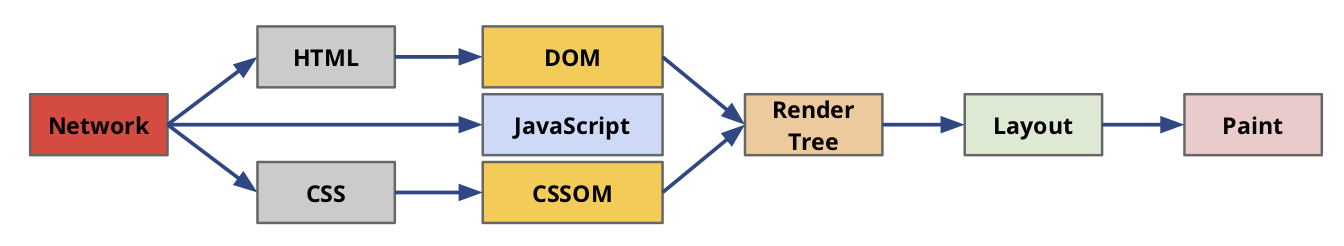
\includegraphics[width=0.7\textwidth]{crp.png}
\caption{Critical Rendering Path}
\label{img:crp}
\end{center}
\end{figure}



% [Single Thread]
%TODO do i need this ?
% How Browsers Work https://developer.mozilla.org/en-US/docs/Web/Performance/How_browsers_work
%- This is somewhat the bottleneck or the technical state of the browser
%- Browser is single threaded
%- Still: Enable smooth interaction: scrolling, responsive to touch, etc.
%- Render time is key
%- Goal: Main thread can complete all the work and still is available to handle user interaction
%-> Improvement: Understand single thread concept of browser and minimize main threads responsibilities
%-> Should lead to: rendering is fast and smooth and responses to interactions are immediate



\paragraph{DOM Construction from HTML}

% [Introduction, Standard]

Once the browser received the first bytes of the HTML file, it starts to parse it into the \textit{Document Object Model} (DOM).
The DOM construction is the first step the browser performs when receiving data.
The DOM is a tree structure and internal representation of the HTML for the browser. % cite https://developer.mozilla.org/en-US/docs/Web/Performance/How_browsers_work
The general parsing process consists of translating from bytes to characters, to tokens, to nodes and finally to the object model.% cite https://developers.google.com/web/fundamentals/performance/critical-rendering-path/constructing-the-object-model
The specification of the DOM is maintained by the WHATWG living standard. % footnote https://dom.spec.whatwg.org/

% The Parsing of the HTML into the DOM is defined in the HTML standard % footnote https://html.spec.whatwg.org/multipage/parsing.html#parsing


% [Render Blocking]

The DOM tree contains information about the content of the document, but not its style.
The styling is defined in the CSS.
Once HTML and CSS are transmitted and processed by the browser, the \textit{Render Tree} can be created, which reflects the actual information and its styling the browser can display.
Within this context, it is possible to categorise resources into render blocking and non-render blocking.
A render blocking resource is a resource that prevents the browser from rendering content to the screen.
HTML and CSS are render blocking resources, as the parsing process of those files blocks the browser of displaying the page to the screen.% cite https://developers.google.com/web/fundamentals/performance/critical-rendering-path/render-blocking-css

% CSS parsing and render tree construction will be discussed below.


% [Incrementally]

As soon as the first data packages of HTML arrive at the browser, the parsing process starts. %cite How Browsers Work https://developer.mozilla.org/en-US/docs/Web/Performance/How_browsers_work
The DOM is created incrementally,  this means that the browser can begin to process the HTML before all of its content is transmitted over the network.


% [Resources]

Usually, within the HTML, external resources are linked which are necessary for the website to be complete, such as CSS or JavaScript.
While parsing the HTML incrementally, eventually a reference to such an external resource will be encountered.
How the external resources CSS and JavaScript are being handled by the browser is discussed below.


%TODO add this?

% How Browsers Work https://developer.mozilla.org/en-US/docs/Web/Performance/How_browsers_work
%- DOM is also exposed, and can be manipulated through various APIs in JavaScript 
%Optimisation: Preload scanner:
%- This process occupies main thread while browser is building DOM Tree
%- parse through the content available and request high priority resources like CSS, JavaScript, and web fonts.
%- will retrieve resources in the background so that by the time the main HTML parser reaches requested assets, they may possibly already be in flight, or have been downloaded




% ------------------------------------------------------------


\paragraph{CSSOM Construction from CSS}


% [Introduction]

The CSS resource contains all information about the styling of the page.
As with the HTML,CSS is converted from bytes to characters, to tokens, to nodes, and finally to the \textit{CSS Object Model} (CSSOM). % cite https://developers.google.com/web/fundamentals/performance/critical-rendering-path/constructing-the-object-model
CSSOM construction is usually very fast . % cite % How Browsers Work https://developer.mozilla.org/en-US/docs/Web/Performance/How_browsers_work
CSSOM is standardized here % footnote https://drafts.csswg.org/cssom/

% The DOM and and CSSOM are separated structures and not yet connected.
% The Render Tree reflects the combination of the two models and will be discussed below.
% Creation of CSSOM happens after DOM is completed. % https://developer.mozilla.org/en-US/docs/Web/Performance/Critical_rendering_path



% [Cascading, Not incrementally]

As opposed to the HTML parsing process, CSS can not be translated to the CSSOM incrementally.
Cause it the cascading nature of style sheets, which has the potential that the styling rules defined at the top of the file may be overridden by rules defined at the very end of the CSS file.
A partial CSSOM is therefore not possible.
Hence the browser needs the entire CSS file before he can create the CSSOM.
%cite  https://developer.mozilla.org/en-US/docs/Web/Performance/Critical_rendering_path


% [Not Parser Blocking]

As soon as the parser encounters a reference to an external style sheet such as

%TODO add caption={} ?
\begin{lstlisting}[language=html, numbers=none]
<link rel="stylesheet" href="styles.css">
\end{lstlisting}

it requests the resource and continues with parsing the HTML.
CSS is not a parser blocking resource.
When the CSS arrived at the browser, the CSSOM construction starts.
%cite  https://blog.logrocket.com/how-browser-rendering-works-behind-the-scenes-6782b0e8fb10/


%TODO add FOUC ?

% https://blog.logrocket.com/how-css-works-parsing-painting-css-in-the-critical-rendering-path-b3ee290762d3/
% - If it just went ahead and rendered to pixels without waiting for the CSSOM we’d see a flash of unstyled content (ugly!) for a moment while the CSSOM was parsing.



% [Render Blocking]

While CSSOM creation is not parser blocking, it is render blocking.
The browser blocks the page rendering until it received and parsed all of the CSS.
Rendering content to the screen is only possible when CSSOM and therefore CSS is available. % cite https://developers.google.com/web/fundamentals/performance/critical-rendering-path/render-blocking-css


% [When finished]

Once the DOM and CSSOM are created, they can be merged together into the render tree, which will be layout and painted to the screen.
Before I describe this process, I will discuss how JavaScript is being handled.


% [Optimization]

%TODO add this: optimization
%- You want to get CSS down to the user as quick as possible:
	%- Inlining styles
	%- Load not needed styles later
%- Optimization: use media queries
%- Better to add styles in single file
%- FOUC: Flash of Unstyled Content: If unstyled content is visible on the screen


% https://developers.google.com/web/fundamentals/performance/critical-rendering-path/render-blocking-css
%Media types and media queries allow us to mark some CSS resources as non-render blocking.


%TODO add this? Lighthouse what is render blocking https://web.dev/render-blocking-resources/
%Lighthouse flags resources as render blocking when:
%A <link rel="stylesheet"> tag that:
%Does not have a disabled attribute. When this attribute is present, the browser does not download the stylesheet.
%Does not have a media attribute that matches the user's device.





% ------------------------------------------------------------



\paragraph{JavaScript in the CRP}


% [Introduction, Parser and Render Blocking]

JavaScript (JS) resources add functionality and interactivity to a web site.
When the browser encounters a script tag such as

%TODO add caption={} ?
\begin{lstlisting}[language=html, numbers=none]
<script src="myScript.js"></script>
\end{lstlisting}

it will stop its current task of parsing, fetch immediately the resource and execute its content, and only then proceed with the creation of the DOM. % cite % Grigorik Conference Talk https://www.youtube.com/watch?v=PkOBnYxqj3k&ab_channel=IlyaGrigorik
See image X.

JS can manipulate and query the DOM tree and directly change the HTML file.
As the HTML file is the input stream for the parser,  the parser stops until the JS is downloaded and executed. % cite https://developer.mozilla.org/en-US/docs/Web/Performance/Critical_rendering_path
Hence JS is parser blocking.
JS fetching and execution stops the parsing of the HTML and the construction of the DOM.
Only after the script finished execution, HTML parsing will continue.

Implicitly, because JS execution blocks DOM creation, and HTML processing itself is render blocking, JS is also render blocking. % cite Grigorik Conference Talk https://www.youtube.com/watch?v=PkOBnYxqj3k&ab_channel=IlyaGrigorik


The behaviour is the same for an external references JS file and a script directly added within in the HTML.


%TODO add this?

% This means that excessive scripts can be a significant bottleneck % How Browsers Work https://developer.mozilla.org/en-US/docs/Web/Performance/How_browsers_work

% https://blog.logrocket.com/how-browser-rendering-works-behind-the-scenes-6782b0e8fb10/
% - If the network is slow, and it takes thousands of milliseconds to fetch app.js, the DOM construction will be halted for the thousands of milliseconds as well

% https://blog.logrocket.com/5-tricks-to-eliminate-render-blocking-resources/
%- You can remove them from the critical rendering path by placing the <script> tags right before the closing </body> tag instead of the <head> section.
%-In this case, they only begin to download after the entire HTML has been downloaded.

% https://developer.mozilla.org/en-US/docs/Web/Performance/How_browsers_work
%- Though the browser's preload scanner hastens this process.


% [Blocked by CSS]

As JS can also manipulate the styling of the page, its execution is blocked until the CSSOM is available.
This means that the execution of the JS is on hold until the CSSOM is ready.
To summarize, while JS blocks the parsing of the HTML to the DOM, JS execution itself is blocked by the creation of the CSSOM.
CSSOM blocks JS, and JS blocks DOM construction. %cite 2013 Grigorik ch 10

Several attributes on the script tag can change the behaviour of the browser.
\textit{Async} and \textit{defer} are options to counter the blocking nature of the script tag.
They will be discussed now.\\



% [async attribute]

With the async (asynchronous) attribute, the browser downloads the JS in the background while continuing with the parsing of the HTML.
The parsing is not blocked and the browser can continue with his task. 
As soon as the JS is downloaded and available,  it is parser blocking: the browser stops the parsing and executes the JS.%cite https://developer.mozilla.org/en-US/docs/Web/HTML/Element/script

The order of all the async scripts within the document is not maintained any more.
Whenever a script is downloaded and available, it will be executed.
It does not matter if an async script was included at the top or bottom of the HTML document. % cite https://blog.logrocket.com/5-tricks-to-eliminate-render-blocking-resources/



% https://blog.logrocket.com/5-tricks-to-eliminate-render-blocking-resources/
%- The async attribute is recommended for independent third-party scripts, such as ads, trackers, and analytics scripts. For example, Google Analytics recommends adding the async attribute to support asynchronous loading in modern browsers.


% [defer attribute]

Like with async, scripts with the defer attribute enable the browser to download the script in parallel while continuing with the parsing of the HTML.
Contrary to async, defer scripts will only be executed after the parsing of the page is complete and the DOM tree is fully constructed,  and the order of the scripts will be maintained.  %cite  https://blog.logrocket.com/5-tricks-to-eliminate-render-blocking-resources/


\begin{figure}[h!]
\begin{center}
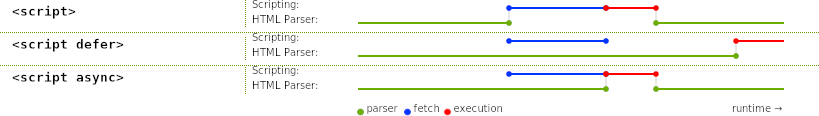
\includegraphics[width=0.8\textwidth]{scripts.png}
\caption{Scripts}
\label{img:latency}
\end{center}
\end{figure}


The async and defer attributes not applicable on inline scripts.
The HTML standard states that  "scripts may specify defer or async, but must not specify either unless the src attribute is present. " % \footnote https://html.spec.whatwg.org/multipage/scripting.html#attr-script-async
As inline scripts do not contain a src attribute, as the source of the script is within the script tags and not external, the async and defer attributes are not applicable.


% https://blog.logrocket.com/5-tricks-to-eliminate-render-blocking-resources/
%- The defer attribute is recommended for scripts that need the DOM, but you want to begin to download them before the document loads, without making them a render blocking resource.
%- You should also use defer rather than async if the document order is important — for instance, when consecutive scripts depend on each other.



% [Transition] ??





% [More stuff]

%TODO add this? preload scanner
% https://developer.mozilla.org/en-US/docs/Web/Performance/How_browsers_work
%- Though the browser's preload scanner hastens this process.

% Grigorik Conference Talk https://www.youtube.com/watch?v=PkOBnYxqj3k&ab_channel=IlyaGrigorik
% And slides https://www.igvita.com/slides/2013/fluent-perfcourse.pdf
%- Asynchronous pattern:
	%- Not the same as async/defer tag
	%- Will fetch JS asynchronously
	%- Uses IIFE which creates a new script tag in the HTML with attribute async
	%see chapter X how Google Analytics is doing this.


%TODO add this? https://web.dev/render-blocking-resources/
%Lighthouse flags resources as render blocking when:
%A <script> tag that:
%Is in the <head> of the document.
%Does not have a defer attribute.
%Does not have an async attribute.


%TODO add this? resource hints
% https://blog.logrocket.com/using-resource-hints-to-optimize-performance/





% ------------------------------------------------------------




\paragraph{Building the Render Tree}


As already described above, HTML and CSS are both render blocking, as they prohibit the rendering of the page.
Rendering can happen once the \textit{Render Tree} is available.
The render tree is the combination of the DOM and CSSOM and captures all visible content with its styles which will be displayed on the screen.
If an element has a CSS property such as \verb|display: none;| it will not occur in the render tree. % cite https://developers.google.com/web/fundamentals/performance/critical-rendering-path/render-tree-construction

The computed render tree is then used to layout the content to the page.


%TODO add this ? Check again when chapter about WPT metrics is done
% 2014 Hogan https://designingforperformance.com/
%Chapter 2
%- Start Render Metric in WPT




% ------------------------------------------------------------


\paragraph{Layout}


In the layout process, the position and size of the nodes from the render tree are calculated.
New layout calculations or reflows are triggered as soon as the screen area changes, e.g. by device rotation or window resizing, or on modifications of the DOM and render tree. % cite How Browsers Work https://developer.mozilla.org/en-US/docs/Web/Performance/How_browsers_work

Once the layout is resolved, the browser continues with painting pixels on the screen.


%TODO add viewport? The projection area is dependent and defined by the viewport

% https://developer.mozilla.org/en-US/docs/Web/Performance/Critical_rendering_path
%- The viewport meta tag defines the width of the layout viewport, impacting the layout.
%- Without it, the browser uses the default viewport width, which on by-default full screen browsers is generally 960px. On by-default full screen browsers, like your phone's browser, by setting <meta name="viewport" content="width=device-width"



% ------------------------------------------------------------


\paragraph{Paint}

Finally, the browser can paint the content on the screen.
If some content changes, browsers are optimized to only repaint areas on the screen affected.  %cite  https://developer.mozilla.org/en-US/docs/Web/Performance/Critical_rendering_path



%TODO add metrics ?
% How Browsers Work https://developer.mozilla.org/en-US/docs/Web/Performance/How_browsers_work
%-> First Meaningful Paint
%- Time to Interactive


%TODO add above the fold?
% https://gtmetrix.com/blog/how-to-eliminate-render-blocking-resources/
%- Above the fold: “Above-the-Fold” refers to the area that the visitor normally sees on a website before scrolling down to see the rest of the content. 


%TODO add performance question?
% https://blog.logrocket.com/how-css-works-parsing-painting-css-in-the-critical-rendering-path-b3ee290762d3/
%- Paint: It’s important to remember that some CSS properties can have a larger impact on the page weight than others (for example, a radial-gradient is much more complex to paint than a simple color).




% ------------------------------------------------------------


%TODO add this ?

% [Continuos Loop, 60 frames per second]

% [Compositing ?]


% ------------------------------------------------------------


\subsection{Technical Background Conclusion}

[tbd]

Network, BE and FE.
Network: Latency and Bandwidth, Navigation steps
FE: CRP

[Link to next section]
Why was this section important for research question?
How is it connected to measurement methods and metrics?


% We could see that performance Metrics are directly derived from this process ??
% Measurement methods will be discussed next
% After that, i will talk about which metrics are available to capture performance data



%TODO add ?
% [Optimizations]

% Grigorik Conference Talk https://www.youtube.com/watch?v=PkOBnYxqj3k&ab_channel=IlyaGrigorik
% And slides https://www.igvita.com/slides/2013/fluent-perfcourse.pdf
%- Optimize the critical rendering path!
%-> styles at the top, scripts at the bottom best practice
% - Different browsers implement different logic for when, and in which order, the individual resource requests are dispatched. As a result, the performance of the application will vary from browser to browser. 2013 Grigorik ch 10



% 2014 Hogan https://designingforperformance.com/
%- Optimizations of CRP:
%- media types and queries on css resources, which makes them non-blocking
%- Load JS efficient
%- Priotize requests for above the fold
%- etc. % Do i need to explain this ??
%Chapter 4:
%CSS and JavaScript Loading:
%- Rules:
%- Load CSS in head
%- CSS blocks rendering
%- Load JS at bottom of the page
%- Load Async
%- JS blocks DOM construction, because browser knows that content from script tag may change Render Tree
%- async tag will execute script once its ready, but order is not berücksichtigt
%- Anything that loads late and changes UI can cause layout shifts
%- 3rd party scripts: Need additional DNS lookup, should not be single point of failure

% https://developer.mozilla.org/en-US/docs/Web/Performance/Critical_rendering_path
%- Optimizing for CRP

% https://medium.com/@luisvieira_gmr/understanding-the-critical-rendering-path-rendering-pages-in-1-second-735c6e45b47a
%- Optimizing

% Grigorik Conference Talk https://www.youtube.com/watch?v=PkOBnYxqj3k&ab_channel=IlyaGrigorik
% And slides https://www.igvita.com/slides/2013/fluent-perfcourse.pdf
%- Async all the things! nice image about async attribute
%- Optimizing DOM:
	%- Minify HTML
	%- Compression
	%- Cache in Browser
%- Unblocking CSS:
	%- Media queries: for responsive design
	%-> Move media queries to separate file
	%- <link rel="stylesheet" href="style-print.css" media="print">
	%-> Will not block rendering
%- Optimizing JS:
	%- Minify, compress, cache
	%- JS is parser blocking
	%- Script tag blocks DOM construction
	%- For external JS, browser waits until JS is fetched and executed
	%- CSS blocks rendering and JS execution
	%- Load and execute script after page is loaded
	%- Page is loaded: Browser fires onload event
	%- Async attribute:
		%- <script src="a.js" async></script>
		%- Does not block CRP (DOM construction, CSSOM)
	%- Inline script blocks CSSOM unless included before CSS request
%- General Strategies:
	%- Minify, compress, cache (HTML, CSS, JS)
%	- Minimize use of render blocking resources (CSS):
	%	- Media queries
		%- Inline CSS
%	- Minimize use of parser blocking resources (JS):
	%	- Defer JS execution
		%- async attribute
%	-> Minimize Bytes
	%-> Reduce critical resources
	%-> Shorten CRP length
	
	
% 2013 Grigorik
%- Browser optimizations...

% 2016 Witt code talks
%- tools available:
%- Profiling: GTMetrix, WebPageTest, PageSpeed Insigths
%- Inlining and Optimization: Critical, PostCSS, processhtml
%- Minification and Compression: Goole Closure, tinyPng, Uglifycss and cssmin

% 2014 Hogan https://designingforperformance.com/
% Chapter 2 The Basics of Page Speed - How Browsers Render Content:
%- Browsers try to parallelize requests for content
%- Requests: Optimizing size and amount of requests has big impact on performance, e.g. get all images in one requests using Sprites

%Page Weight is somewhat important:
%- Sum of all file sizes
%- Averages in httparchive, which i also used in one approach % https://httparchive.org/reports/state-of-the-web?start=latest

%Other Impacts on Page Speed
%- "environmental factors"
%- Geography, CDNs
%- Network
%- Browser


% 2016 Witt code talks
%- Possible Improvements:
%- HTTP2
%- Avoid redirects
%- Caching headers
%- CDNs
%- Single Page Apps


%TODO add this ??
% [JavaScript Parsing]
% https://medium.com/reloading/javascript-start-up-performance-69200f43b201






% ---------------------------------------------------------------------------------------------------------------------------------------
% ---------------------------------------------------------------------------------------------------------------------------------------
% ---------------------------------------------------------------------------------------------------------------------------------------
% ---------------------------------------------------------------------------------------------------------------------------------------


\section{Measurement Methods}


[tbd]


% [Introduction]

Last section: At this point we have an understanding of how web sites are being loaded into the browser and displayed to the user.
Some of the steps are more important for performance than others.
In this section, I will describe how to measure the performance of a website.


[Link to Research Question]

% add some more info for Roter Faden, why is this here? whats all about ?
% start with web analyitcs and web performance context
% as described in section web analytics, measurement is important...
% i could also motivate here that i will use both methods in my experiment thats why i need to explain them here


% [Methods]

Multiple methods for measuring website performance exist.
The prominent ones are synthetic monitoring and real user monitoring.
They will be discussed below.

Some other methods are mentioned in the last section.

After discussing measurement methods, I can finally discuss the metrics we want to measure.




% ----------------------------------------------------------------------------------------------



\subsection{Synthetic Monitoring}


\subsubsection{The "Synthetic" Aspect in Synthetic Monitoring}


As the name already suggests, synthetic monitoring is a measurement method performed in an artificial, laboratory-like, synthetic environment.
Test agents simulate real users and are configured to run a browser, load the web site under observation while capturing performance data.
Synthetic monitoring does not take real user traffic into account. % cite 2015 cito

Performance data can be captured using common performance APIs as described in section X.
Additionally, through video recording and analysis,  user centric metrics such as Speed Index can be computed (see section X.) % cite 2021 Wolle 

In synthetic monitoring, many possible configurations and variables of the test agent (client) are under control, such as the location (geography), network conditions, device type, browser version, and so on. % cite https://developer.mozilla.org/en-US/docs/Web/Performance/Rum-vs-Synthetic
Hence, the tester has control over many variables that impact performance. %and can use this to test impact of variables...

The controlled environment makes it possible to capture performance data for a specific set up of configurations, such as the test agents location or browser version, which may help to identify issues regarding certain user segments.  For example., a test could check the performance of all users using Firefox running on macOS in Germany. % cite 2009 Croll

Apart from defining the technical configuration such as browser version or network condition, the tester can also define artificial user journeys to simulate real user behaviour. % cite 2021 Wolle

A characteristic of the controlled environment is that measured data and test results are rather consistent with low variability and can therefore provide a performance base line for the web site under observation and facilitate performance tuning.% cite 2013 Meenan


\paragraph{Synthetic Monitoring is not about Real Users}

Synthetic monitoring does not capture data of real users as the web sites traffic is generated artificially.
Real user behaviour is approximated through simulation of users by for example predefining user paths.
The measured performance data does not necessarily reflect actual real user experience and the tester should not assume that "synthetic results are like real-user metrics". %cite 2016 Viscomi

Capturing the wide variety and diversity of real-world users such as which pages they visits,, the general configuration of the users machine such as the CPU, GPU and memory performance, what data stores the browser cache and which browser version is being used, the screen size, the operating system, and the network connection to name a few, is difficult to represent in synthetic monitoring. % cite 2013 Meenan, 2013 Grigorik
The selected test configuration in synthetic monitoring only reflects one special use case and can only approximate what a user with a similar set up may experience. % cite 2016 Viscomi
In short, synthetic monitoring test results "are synthetic and therefore not representative for actual user data".  % cite 2021 Wolle



\subsubsection{The "Monitoring" Aspect in Synthetic Monitoring}


Synthetic monitoring can be automated and used to monitor a systems performance in real time while generating up to date reports for the systems maintainer. % cite https://developer.mozilla.org/en-US/docs/Web/Performance/Rum-vs-Synthetic
Monitoring enables to check the availability of the web site around the globe, %cite 2009 Croll
to identify performance issues before real users are aware of them. % cite 2013 Grigorik https://hpbn.co/primer-on-web-performance/
and is in general helpful for continuous "health checks" of the running system. %cite  2021 Wolle 

As any web site can be tested synthetically, it is possible to compare performance data across multiple competitors. % cite 2009 Croll


% [Tools]

Many synthetic monitoring tools exists (For a list of tools, see for example 2016 Kaur or some online resources here).
WebPageTest is one of them and will be discussed in section X.


% [Transition]

Coming back to e-commerce context, as discussed in section X.  a online shops performance correlates with the revenue.
Synthetic monitoring allows to capture performance metrics independent of real user behaviour.
Real user behaviour is not measured in synthetic monitoring.
As only real users are capable of generating revenue, synthetic monitoring can not identify correlations between user satisfaction and performance (as described in section X.).%cite  2021 Wolle blog post https://medium.baqend.com/mobile-site-speed-measurement-best-practices-ff4a3f91b003

In order to do this, RUM is needed.
Real-User Monitoring (RUM) enables to capture data of each individual real user .
RUM will be discussed next.



%TODO cut out google lighthouse completely ?
%- Google Lighthouse


%TODO add waterfall ?
% 2021 Wolle blog post https://medium.baqend.com/mobile-site-speed-measurement-best-practices-ff4a3f91b003
%- waterfall diagram contains timing information on when the individual resources were requested, from which domain and over what kind of connection each of them was served, and how long transmission took


% 2016 Viscomi
%- synthetic tools are deliberately designed to focus on the performance of a web page under strict conditions that are otherwise highly volatile in real-user performance


% 2021 Wolle blog post https://medium.baqend.com/mobile-site-speed-measurement-best-practices-ff4a3f91b003
%- Modern tooling also tells you when the browser was actually doing useful work (e.g. rendering) and when it was idle and waiting for loads to finish




% ----------------------------------------------------------------------------------------------
% ----------------------------------------------------------------------------------------------



\subsection{Real-User Monitoring}


%\subsubsection{Measurements with Real Users}

As the name suggests, Real-User Monitoring (RUM) is about collecting and measuring data from real users visiting the web site.
As opposed to synthetic monitoring, where web site traffic is generated artificially and performance experience from real users is only approximated, RUM data relies on real user traffic and captures data directly from each users browser. 
RUM measures the performance as experienced by the users. % cite https://developer.mozilla.org/en-US/docs/Web/Performance/Rum-vs-Synthetic



\subsubsection{The Page Tagging Technique in RUM}

% [Page Tagging]

As already described in section X. Page Tagging is a technique to instrument the users browser in order to collect data and report it back to an analytics server.
RUM is based on page tagging, in terms of that it relies on a JS code snippet (tracking or code) which will be loaded into the users browser.
Once this JS code is loaded and executed in the browser, it collects data and sends it back to an analytics service.
If the user blocks JS, or the script can not be downloaded due to other reasons,  RUM will not work.
Once the data arrives at an analytics service, is has to be stored and an interface for the analyst has to be provided in order that he can query the data and get insights, for example by providing a dashboard. %cite 2021 Wolle blog post https://medium.baqend.com/mobile-site-speed-measurement-best-practices-ff4a3f91b003

As RUM relies on the JS code, the very first opportunity to measure data is when this JS code has been downloaded and executed.
Anything what happens before this step is not visible for the tracking script and therefore the analyst.
Meenan states that approximately 20 \% of the loading process lies outside of the RUM measurement scope and "getting a reliable start time for measurements from the real world has been the biggest barrier to using RUM".% cite 2013 Meenan

Another facet of RUM is that ideally the measuring of data has as little as possible impact on the web sites rendering process and that network capacity should not be occupied by RUM scripts and block resources of the CRP (see section X.) % cite  2021 Wolle blog post https://medium.baqend.com/mobile-site-speed-measurement-best-practices-ff4a3f91b003
If RUM, as a page tagging technique, is slowing down the web site under observation, is one research question of this thesis.
The evaluation of the controlled experiment tackling this questions states that RUM...., as discussed in great detail in section X. %TODO add conclusion of evaluation here


% [Diversity of Users and Data]

RUM is independent of the users set up or environment and collects data for all active users:
Regardless of the device, the browser,the network condition or the geographical location of the user, as long as the measurement script is downloaded into the users browser, RUM collects data.% cite https://developer.mozilla.org/en-US/docs/Web/Performance/Rum-vs-Synthetic
Hence, RUM data represents each individual user experience. % cite 2016 Viscomi

Through the diversity of users and the unique environment of each user,  RUM data tends to be more diverse and heterogeneous than data collected by synthetic monitoring. % cite 2013 Meenan



\subsubsection{RUM Measures Behaviour of Real Users}

%TODO here i need to introduce maybe in e-commerce again? Or what is the roter faden? like funnel analysis all this stuff reference it here?

% [E-Commerce Background]

As discussed in section X, a web sites performance and user satisfaction are directly correlated.
A critical part of RUM is to not only capture performance metrics, but also measure user behaviour, for example how the user interacts with the web site and where he clicks. %cite 2021 Wolle blog post https://medium.baqend.com/mobile-site-speed-measurement-best-practices-ff4a3f91b003
In an e-commerce context, user behaviour questions of interest are for example if a new campaign changes user behaviour as expected or where users leave the check out process. %cite 2021 wolle and % https://developer.mozilla.org/en-US/docs/Web/Performance/Rum-vs-Synthetic

RUM facilitates the combination of collected metrics with user behaviour and business KPIs and can answer questions such as if and how the performance of the web site affects the user behaviour, for example if users buy more or less depending on the web sites speed.% cite Eggplant whitepaper
Thus RUM is not only important for understanding user behaviour, but also for optimizing the web site and to increase revenue.
With techniques such as cookies (see section X.), it is also possible to track user behaviour not only for one page load but over a series of web site visits, leading to even more detailed insights about the visitor. %cite 2021 Wolle blog post https://medium.baqend.com/mobile-site-speed-measurement-best-practices-ff4a3f91b003


% [Tools]

Multiple RUM tools and JS libraries exists, such as Boomerang by Akamai. \footnote{\url{https://github.com/akamai/boomerang} [23.06.2021]}
The main player Google Analytics will be discussed in greater detail in section X.

% SpeedKit ?


% [Transition]

Google collects RUM and browser data of chrome users agreed to do so.
The data is accessible through the Chrome User Experience Report (CrUX) and will be discussed next.



%TODO add this here?
% [Performance Data]

%Which data and metrics RUM can collect and measure is discussed in greater detail in section X.
%A part from metrics exposed by Web APIs or own implementations
%RUM can also gather data about the users device, operatins system or geographic location. %cite 2015 Cito
%The performance data and timings are exposed through a variety of APIs which the JS tracking code has access to.

% 2013 Grigorik https://hpbn.co/primer-on-web-performance/
%- APIs to measure real users (will be discussed in metrics chapter):
%- Navigation Timing
%- Resource TIming
%- User TIming
%- The combination of Navigation, Resource, and User timing APIs provides all the necessary tools to instrument and conduct real-user performance measurement for every web application

% Cito
%- Real-User Monitoring leverages browser APIs to collect data specific to each end-user transaction

% 2021 Wolle blog post https://medium.baqend.com/mobile-site-speed-measurement-best-practices-ff4a3f91b003
%- Collected information includes various timers to capture network and rendering performance
%- To also capture details about the user’s device and browser or on the referring website over which the user arrived, the user agent string and other data artifacts are collected along with the values obtained from the Navigation and Performance Timing APIs


% [Business Data]

%conversion rates etc.






% ----------------------------------------------------------------------------------------------



\subsubsection{Chrome User Experience Report (CrUX)}


The Chrome User Experience Report (CrUX) is a RUM method implemented by Google which collects real user data of Chrome users.
As soon as the Chrome user gives his consent, data collection can start and does not need any more set up.

The CrUX only captures data from Chrome users and is therefore not an exhaustive sample of the web users population, as data by users browsing the web with for example Firefox or Safari is not collected.
% cite 2021 Wolle blog post https://medium.baqend.com/mobile-site-speed-measurement-best-practices-ff4a3f91b003

The collected data is available via Googles PageSpeed Insights, the CrUX Dashboard or the BigQuery and CrUX API. % cite https://developers.google.com/web/tools/chrome-user-experience-report


%TODO add here which metrics it collects?



% ----------------------------------------------------------------------------------------------


\subsection{Log Files and Surveys}

[tbd]

Other methods are surveys and log file analysis.

% 2021 Wolle blog post https://medium.baqend.com/mobile-site-speed-measurement-best-practices-ff4a3f91b003

%Log analysis:
%- concerned with technical performance in the backend
%- generates insights from the data that is already available from the application server, proxy, or content delivery network (CDN)
%- TTFB
%- Server logs typically only reflect the time it took to send the first response, not until the client actually started receiving it
%- Analyzing logs from application servers, CDNs, or proxies is a reasonable first step to discover potential bottlenecks, but it only covers the server side and does not provide any information on client-side processing in general or rendering performance in particular


%Surveys:
%- directly ask the users for their opinions
%- direct approach to understanding whether or not users are satisfied with website performance: Just ask them for their opinion
%- online surveys or by offering some sort of price or chance to win a competition in exchange for the users opinions. 
%- Other options include actual interviews or monitoring users in a lab setting to find out how they react while surfing on the website.
%- they only cover a small sample of the user base and therefore may be subject to a certain selection bias
%- user perception can be highly inaccurate
%- Getting reliable info from user surveys is therefore no trivial task
%- some forms of surveys (e.g. lab experiments) can be relatively expensive to conduct in comparison to some of the fully automated alternatives for collecting information
%- are great for collecting qualitative feedback on the user experience, but are not suitable for gathering quantitative measurements



% ----------------------------------------------------------------------------------------------



\subsection{Measurement Methods Conclusion}


Multiple methods to measure performance of a web site exist.
Two main complementary techniques exist, Synthetic Monitoring and Real-User Monitoring.

Synthetic Monitoring measures a web sites performance in a controlled environment using test agents and is especially useful to find a performance base line of the web site and for continuous monitoring and health checks.
Performance as end users may experience it can only be approximated it is not captured by synthetic monitoring.

RUM collects data from each user visiting the web site and reports it back to an analytics server.
RUM is especially useful when combining multiple metrics together such as performance and business metrics in order to analyse user behaviour.
On the other hand, when no user is visiting the web site, RUM is not collecting any data.

Other performance measurement methods such as CrUX and surveys provide browser specific or quality data and complement the analysts tool box.


\begin{table}[h!]
\begin{center}
\begin{tabular}{  c | c  }
Synthetic Monitoring & RUM \\
\hline
\hline
Artificial test agents & Real users \\
\hline
Controlled configuration & No control over configuration \\
\hline
Approximates real user data & Collects real user data \\
\hline
For monitoring & Links user behaviour to business KPIs \\
\end{tabular}
\caption{Synthetic Monitoring and RUM}
\end{center}
\end{table}


% [Metrics, Transition]

Metrics are critical in order to map performance to some sort of value or number.
Through metrics, performance is quantifiable to some extent and therefore comparable.

As already described, measurement methods such as synthetic monitoring or RUM can measure metrics such as "performance" or "business" metrics.
What are does metrics exactly?
What do they reflect?
How can they be measured?

Those questions will be addressed in the next section.





% --------------------------------------------------------------------------------------------------------------------------------------------
% --------------------------------------------------------------------------------------------------------------------------------------------




\section{Metrics}


[tbd]


[Link to Research Question] \\

% roter faden: motivate with context web analytics, web performance, user satisfaction etc



% [Quantification and Analysis]

Through metrics, performance is quantifiable, as metrics reflect performance in numbers.
Once performance is mapped to numbers, they can be compared with each other, for example over time, after a change in the measured application,  or with numbers of a competitor. % cite https://developer.mozilla.org/en-US/docs/Learn/Performance/Measuring_performance
Through their performance quantification, metrics facilitate the analysis of website traffic.
Specific metric values can be used as a target for goal achievement and are therefore a critical instrument for improving websites. % cite 2009 Jansen
Ideally, metrics are precise and serve as objective criteria for the evaluation of the measured website. % cite https://web.dev/user-centric-performance-metrics/


%TODO add this ?
% https://speedcurve.com/blog/rendering-metrics/
%- Metrics quantify behavior
%- we're trying to capture the behavior of a website in terms of speed and construction
%- statistics about how the site is built such as number of HTTP requests, size of stylesheets, and DOM depth
%- Speed is tracked by time-based metrics that capture when things happen during the user's experience with the website: start render, DOM interactive, page load, etc. 



% [Relevance]

The selection of metrics and accordingly their relevance for the website is crucial.
Just as each website is unique and serves a different purpose, so should metrics be, which quantify the website.
It is important to measure what is important and relevant for the users and reaching business goals, while "each business has its own definitions of success". % cite 2009 Croll p 7,  https://developer.mozilla.org/en-US/docs/Learn/Performance/Measuring_performance
Hence, metrics are ideally tailored and custom to the website and they should track if "your business benefited in some way from their [the users] visits." % cite 2009 Croll p 15



% [Usable]

Metrics are only helpful when they are useful.
That implies that the collection and measurement of metrics should be consistent and their representation should be unser-friendly and understandable. % cite https://developer.mozilla.org/en-US/docs/Learn/Performance/Measuring_performance
Kumar states that ideally, good metrics are uncomplex, relevant, timely, and instantly useful.  \\% cite 2012 Kumar


% [Section Outline]

In the next section, I will describe metrics which are more likely correlated and mapped to business topics, such as conversion or bounce rate.
I use the term "business" or "non-performance" metrics to draw a line between metrics mainly concerned with a websites performance and metrics reflecting other web analytics aspects.
Business metrics are not directly responsible to capture performance data such as loading speed of a website.

After discussing non-performance metrics, performance metrics are described.
This includes metrics concerned about page weight, load timings, and user-perceived performance.

Finally, custom metrics are discussed.


%TODO add this ?
% Summary / Metrics Taxonomy



%TODO add this ?

% 2019 Enghardt
%"metrics as well as experiments have to realistically reflect possible performance improvements for actual users"

% [Metrics and KPIs]

% 2015 Bekavac



% ------------------------------------



\subsection{Business or "Non-Performance" Metrics}


As already described, the term business metrics should subsume metrics which are not directly concerned with capturing site speed or user-perceived performance.
Business, or non-performance metrics, collect data about any aspect of a website which is of interest for the analyst.
Thus, theoretically an unlimited amount of metrics exist, as also for each specific questions, custom metrics are made up.

In literature, a core corpus of metrics can be found and multiple ideas of structuring and categorizing those metrics exist.
The different possibilities of categorizations are discussed next.
Afterwards, one approach of categorization is then used to list a selection of common business metrics.




% ------------------------------------


\subsubsection{Possible Categorizations of Business Metrics}


Categories help to better grasp and comprehend metrics, and they can provide structure and order.
Following are some examples of business metrics categorizations as they are presented in literature.

Peterson arguments from a marketing perspective and categorizes the metrics according to the customer life cycle, which includes the phases reach, acquisition, conversion, and retention. % cite 2004 Peterson

Metrics for measuring \textit{Reach} are for example number or percentage of new visitor.
\textit{Acquisition} contains metrics such as average number of visits per visitor or average pages viewed per visitor.
The category \textit{Conversion} includes metrics such as conversion or abandonment rates.
And the last category \textit{Retention} includes metrics such as the number of returning visitors.
This proposed categorization is highly customer-related and customer-centric and from a marketers perspective. 

%Reach:  - Overall Traffic Volumes,  Number of Visits
% Measuring Acquisition: - Percent New Visitors, - Average Number of Page Views per Visit
  
The Web Analytics Association defines three types and accordingly categories of metrics: \textit{Counts}, \textit{Ratios} and \textit{KPIs},% cite 2007 Burby
Where counts are metrics which are single numbers like the number of visits, ratios consist of counts divided by other counts, such as page views per visit.
KPIs are counts or ratios with a specific meaning and importance for the specific business.

Jansen defines four categories for web analytics metrics: % cite 2009 Jansen p.30
\textit{Site Usage}, which encompasses metrics such as demographics and system statistics, but also visitor length and type,
\textit{Referrers}, that are metrics describing the referring URL,
\textit{Site Content Analysis}, which includes metrics such as top pages or visitor paths, and
\textit{Quality Assurance} with metrics reflecting errors or other quality aspects of the measured system.

% Site usage: Internal Search Information
% Referrers: keyword Analysis	
	 
Croll arguments that all metrics answer at least one of four user-centric questions: \textit{What did they do?}, \textit{How did they do it?,} \textit{Why did they do it?}, and \textit{Could they do it?}. % cite 2009 Croll
Accordingly, the metrics are categorised by the question they answer.

Bekavac organizes the metric according to what they describe: \textit{Visits}, such as entry or exit page,
\textit{Visitors}, such as the metrics capturing new or returning visitors,
metrics such as page exit ratio or bounce rate which describe \textit{Visitor Engagement},
and metrics describing \textit{Conversions} as the conversion rate. % cite 2015 Bekavac

%visits: entry page, landing page, exit page, visit duration, referrer, ctr
%- For describing Visitors: repeat visitor, visits per visitor, recency, frequency
%- For describing Visitor engagement: page exit ratio, bounce rate

Hassler proposes a classification which is close and similar to the WAA proposed categorisation.
The metrics are ordered by their type: % cite 2017 Hassler
\textit{Counts} are absolute values like visitors or total sales,
\textit{Relations} put counts into relation for example as percentages, such as page views per visitor,
and \textit{Values} include non-numerical metrics such as referrer or search term.

Gessert et al.  propose a semantic categorization of metrics, they structure the metrics according to their meaning and their domain membership.
The categories are \textit{Performance}, which includes performance metrics such as Time to First Byte or First Input Delay (see section X.), \textit{User Engagement} metrics such as the session length or the bounce rate, \textit{Business KPIs} such as the cart size or the amount of transaction, but also conversion rates and revenue, and \textit{QA Metadata} which subsumes technical metrics like JS errors or the browser distribution.% cite 2020 Wolle https://www.youtube.com/watch?v=avPcOFzUa1Q&ab_channel=WolframWingerath

%- User Engagement: Session Length, First user interaction
% QA Metadata: Page views and sessions, Caching insights


%TODO add?
% 2004 Phippen
% 2020 Heinemann 4.1.4
%Metrics Categories for E-Shop:
%- Attraction
%- Acquisition
%- Retention
%- Umsatzleistung
%- Warenleistung
%- Ergebnisleitung

%- also customer life cycle

\begin{table}[h!]
\begin{center}
\begin{tabular}{  c | c  }
Value-Driven & \{Counts, Ratios, KPIs\},  \\
 & \{Counts, Relations, Values\} \\
\hline
Semantic-Driven & \{Performance, User Engagement, Business KPIs, QA Metadata\},  \\
& \{Site Usage, Referres, Site Content Analysis, Quality Assurance\} \\
\hline
Marketing-Driven & \{Reach, Acquisition, Conversion, Retention\}, \\
& \{Visits, Visitors, Visitor Engagement, Conversions\} \\
\end{tabular}
\caption{Business Metrics Categorizations}
\end{center}
\end{table}



% [Conclusion]

As described above, multiple categorizations of metrics are proposed in literature.
While some authors group the metrics by their type of value, e.g. if they count something or represent a ratio, others use a more semantic approach and group the metrics by their meaning, with some extreme examples by authors which group only through a marketing perspective.
% Orthogonal to semantic: "number" categorization: Count, ratio, ...

In the following, I will list some metrics and provide brief explanations, following the categorization of counts,ratios and values.
After that, i will take a look at metrics which are specific for performance.



%TODO add ?
% Customer Life Cycle and Pyramid
% 2004 Peterson
%Pyramid Model described the data itself and not metrics
%Metrics categorised by customer life cycle: Reach, Acquisition, Conversion, Retention

% 2008 Reese
%- Pyramidenmodell 




% ---------------------------------------------------------------


\subsubsection{Business Metrics Examples}


Table X provides web analytics metrics which are not directly concerned with performance.
The categories used to structure the metrics are \textit{Counts}, \textit{Ratios} and \textit{Non-Numerical Values}, like they are already defined by Hassler or WAA in the section above. % cite ?

%TODO even add this? already described above
% [Counts]
%Counts hold a value describing how many 
%Counts can be measured over time: last hour, month, from to, etc.
%Averages are possible
%Compare with Segmentation

% [Ratios]
%Ratios are a combination of numerical values.
%As Ratio or Percentage

% [Non-Numerical Values]
%Non-Numerical Values can not be reflected as a number.


\begin{center}
	\small
	\begin{longtable}{ | p{0.3\linewidth} | p{0.6\linewidth} | }
	
	\hline
	\multicolumn{2}{|c|}{ \cellcolor{lightgrey} Counts} \\
	\hline
	Hits & Represent amount of requests to the server.  \\ % 2004 Peterson
	\hline
	Visits or Sessions & Count how many users view the website \\ % 2004 Peterson
	\hline
	Session Length & How long the session endures \\ % 2007 Burby
	\hline
	Page Views & How often a page has been viewed \\ % 2004 Peterson
	\hline
	Single Page Visits & Sessions where one page has been viewed \\ % 2007 Burby
	\hline
	New / Unique / Repeat / Return Visitors & ... \\
	\hline
%	Time on Page & ... \\
	%\hline
%	Time between Visits & ... \\
%	\hline
	JS Errors & How many JS errors occured \\
	\hline
	Cart Size & ... \\
	\hline
	Conversions & ...  (business specific) \\
	\hline
	\textit{etc.} &  \\

	\hline
	\multicolumn{2}{|c|}{ \cellcolor{lightgrey} Ratios} \\
	\hline
	Conversion Rate & ... \\
	\hline
	Bounce Rate & ... \\
	\hline
	Abandonment Rate & ... \\
	\hline
	Page Views per Visitor & ... \\
	\hline
	New Visitors Percentage & ... \\
	\hline
	Visits per Visitor & ... \\
	\hline
	Page Exit Ratio & ... \\
	\hline
	Click Through Rate (CTR) & ... \\
	\hline
	\textit{etc.} & \\	
	
	\hline
	\multicolumn{2}{|c|}{ \cellcolor{lightgrey} Non-Numerical Values} \\
	\hline
	Demographics & ... \\	
	\hline
	Referrer & ... \\	
	\hline
	\textit{etc.} &  \\
	\hline
	
	\caption{Business Metrics Examples} % needs to go inside longtable environment
	\label{tab:businessmetrics}
	\end{longtable}
\end{center}


%\paragraph{Hits}
% 2004 Peterson
% 2017 Hassler


%\paragraph{Visits}
% 2004 Peterson
% 2007 Burby
% 2009 Waisberg
% 2017 Hassler

%\paragraph{Session Length}
% 2007 Burby


%\paragraph{Page Views}
% 2004 Peterson
% 2007 Burby
% 2009 Croll p. 74 Page View, first useful web analytics metric
% 2009 Waisberg
% 2015 Zheng
% 2017 Hassler


%\paragraph{Single Page Visits}
% 2007 Burby

%\paragraph{New Visitors}
% 2004 Peterson
% 2007 Burby

%\paragraph{Unique Visitors}
% 2004 Peterson
% 2007 Burby
% 2017 Hassler

%\paragraph{Repeat Visitors}
% 2007 Burby

%\paragraph{Return Visitor}
% 2007 Burby

%\paragraph{Time on Page}
%\paragraph{Time between Visits}

%\paragraph{JS Errors}

%\paragraph{Cart Size}
% 2009 Croll p 24 in site effectiveness

%\paragraph{Conversions}


% -------------- RATIOS --------------


%\paragraph{Bounce Rate}
% 2007 Burby
% 2009 Waisberg

%\paragraph{Conversion Rate}
% 2004 Peterson

% 2009 Croll
%- The percentage of visitors that your site converts to contributors, buyers, or users is the most important metric you can track

%\paragraph{Abandonment Rate}
% 2004 Peterson
% 2009 Croll

%\paragraph{Page Views per Visitor}
% 2007 Burby
% 2009 Waisberg

%\paragraph{New Visitors Percentage}
% 2009 Waisberg


%\paragraph{Visits per Visitor}

%\paragraph{Page Exit Ratio}
% 2007 Burby


%\paragraph{Click Through Rate (CTR)}
% 2004 Peterson
% 2007 Burby
% 2009 Croll



% % -------------- NON_NUMERICAL_VALUES --------------


%TODO find some more examples here

%\paragraph{Demographics}
%age, gender, browser, geography, ...

%\paragraph{Referrer}
% 2004 Peterson
% 2009 Croll



% --------------------------------------


% [Transition]

The table X provides a selection of common business metrics, following the proposed categorization of counts, ratios and non-numerical values and is not complete.
In the next section, I will discuss metrics which are designed to directly capture performance related data.


%TODO even add this? outline can be made in beginning of next section
%As performance is directly connected to time, most of those performance metrics are measuring a timestamp.
%Some are also displaying a score. 
%This will be discussed.



%TODO should i show how to actual measure those metrics, like visits, hits, conversion rate etc ?


% Kessler 2012 -> dont have this digital...
% Erfolg messen und bewerten
 %Traffic:
%	 Page Impression / Page View
%	 Visit
%	 Visitor / Unique visitor
% Bounce rate
 %Conversion rate
 %CTR: Click-through-rate
 %Session length
 
 
 % 2016 Kollewe -> nicht digital
% Besucheranalyse: Wie viele Besucher?, Anzahl Besucher mit Mobilgerät, Demographische Daten (Geschlecht, Altersgruppe)
% Seitenanalyse: Was machen die Besucher im Shop?, Zielseite / Startseite: Erste Seite, die ein Besucher angeschaut hat, Ausstiegseite
% E-Commerce-Analyse: Transkations-daten aus Shop, Funnel-Analyse



% --------------------------------------------------------------------------------------------------------------------------------------------
% --------------------------------------------------------------------------------------------------------------------------------------------



\subsection{Performance Metrics}

Business or non-performance metrics track data about a lot of different aspects and topics, for example metrics about how many visitors the website has or what the conversion rate is.
For measuring performance, for example site speed and how users perceive the performance of the website, a set of special metrics is needed.
Performance metrics are established to measure various performance aspects of a website and will be discussed in this section.

%TODO add this?
% No official definitions, lack of definitions (enghardt)
% Still there are informal standard
% Implementation can vary between tools who measure metrics


% [Outline]

As with business or non-performance metrics, multiple ways exist to structure and categorize performance metrics.
One way to order performance metrics is to differentiate between performance timing metrics, which measure elapsed time for concrete processes and navigation steps from the CRP, and user-centric performance metrics, which approximate user perceived performance by visual analysis.
Both classes of metrics will be discussed in the following.
But before I will talk about metrics regarding page weight and size of the website.
A characterization of custom metrics concludes the section about performance metrics.



% -----------------------------------------------------------------------



\subsubsection{Page Weight}

A naive approach of quantifying a website is measuring its size and the amount of resources needed to build the website.
Page weight can be used as a performance metric as the performance of a website depends on the network condition, like download speed and latency.
The more bytes have to be transmitted over the network, the longer it takes for the website to get constructed and the longer the waiting time for the user.
Similar for requests, the more requests are needed, more connections need to be established, which takes more time.

A website consists of multiple resources, such as HTML files, fonts, script files or images (cf. table X).
Page weight describes the number of bytes fetched and requests made for each resource type. %compare cite HTTP Archive

\begin{center}
\begin{tabular}{| c | c | c | c | }
\hline
HTML & CSS  & JS & Fonts \\
\hline
Images & Videos & Others & (Total) \\
\hline
\end{tabular}
\end{center}
%TODO add caption

Page weight is a first assessment for a website regarding performance.
It is mainly useful for comparison with median values or other websites, but has little to nothing expressiveness and significance for evaluating a websites performance.
To get more useful insights about a websites performance, other metrics are in need, such as performance timings metrics, which will be discussed in the next section.
As described in section X,  the idea of page weight is used to construct a test site with a median page weight values.


% -----------------------------------------------------------------------


\subsubsection{Navigation Timing Metrics}

Navigation timing metrics depict elapsed time within the website loading process such as navigation and CRP (cf.  section X).
They are calculated and derived from a set of standardized Web APIs.
In the following, I will briefly explain the nature of web standards and recommendations.
Then, performance relevant specifications and the metrics they expose are discussed.


\paragraph{Web Standards}

Web Standards are documents describing the technology used to build the WWW. % cite https://developer.mozilla.org/en-US/docs/Learn/Getting_started_with_the_web/The_web_and_web_standards
Those documents, also called specifications, are maintained by different groups and organizations.
Multiple organizations exist to provide and maintain standards for different areas and technologies of the web.
Such organisations are for example the WHATWG, which maintains the HTML living standard\footnote{\url{https://whatwg.org/} [11.07.2021]}, or Ecma International, providing the specification for JS.\footnote{\url{https://www.ecma-international.org/} [11.07.2021]}.

The World Wide Web Consortium (W3C) is an organization which maintains different standards for the WWW, including specifications for performance measurement\footnote{\url{https://www.w3.org/} [11.07.2021]}, and will be discussed next.


\paragraph{W3C}

% [What is W3C]

The W3C was founded in 1994 by Tim Berners-Lee, with the goal to bring together "representatives from many different technology companies to work together on the creation of web technology specifications". % cite https://developer.mozilla.org/en-US/docs/Learn/Getting_started_with_the_web/The_web_and_web_standards
The W3C maintains and publishes documents that describe and define web technologies such as DOM, SVG or CSS. % cite https://www.w3.org/standards/faq


% [Recommendation Process]

The document, or specification creation, follows a "recommendation track", which describes the hurdles a document needs to overcome in order to turn from an idea into a final recommendation and web standard, which browser vendors implement as concrete APIs. %cite  https://www.w3.org/2020/Process-20200915/#rec-track
The phases in the recommendation track are described by "maturity levels" of the document and are as follows:
First Public Working Draft (FPWD) $\,\to\,$ Working Draft (WD) $\,\to\,$ Candidate Recommendations (CR) $\,\to\,$ Proposed Recommendation (PR) $\,\to\,$ W3C Recommendation (REC).  % cite https://www.w3.org/2015/Process-20150901/#maturity-levels
W3C Recommendations are considered to be web standards. % cite https://www.w3.org/standards/faq

%TODO maybe draw some nice graphic for the recommendation track ?


\paragraph{Web Performance Working Group}

% [Introduction]

Within the W3C, several groups exist, each one concerned with a specific topic within the WWW universe. % cite https://www.w3.org/groups/wg/
The Web Performance Working Group, founded in 2010, is a group responsible "to provide methods to measure aspects of application performance of user agent features and APIs" \footnote{\url{https://www.w3.org/webperf/} [11.07.2021]}.

% [Specs]

The Web Performance Working Group publishes and maintains a variety of documents concerned with performance measurement, such as High Resolution Time, Navigation Timing or Page Visibility. % cite https://www.w3.org/groups/wg/webperf/publications
The released publications especially important for performance metrics are discussed next.


%TODO add this ?

% https://www.w3.org/2021/02/webperf.html
%- Working Groups push new recommendations and invent them
%Web Performance Working Group is responsible:
%- Measurement
%- Scheduling
%- Adaptation
%-> Important is Measurement


%Server Timing:
% https://www.w3.org/TR/server-timing/

% https://w3c.github.io/perf-timing-primer/#dfn-time-origin
%- attempt to address the concern about lacking insight into how or why certain stages of the request-response cycle have taken as much time as they have


%others, not important for metrics:
%- Beacon
%- Cooperative Scheduling of Background Tasks
%- Device Memory
%- Reporting
%- Network Error Logging


% and some unofficial drafts
% Network Information API (not official w3c) https://wicg.github.io/netinfo/
% Element Timing API (not official w3c) https://wicg.github.io/element-timing/
% Event Timing API (not official w3c) https://wicg.github.io/event-timing/



% -----------------------------------


\paragraph{High Resolution Time}

Two versions of High Resolution Time exist.
High Resolution Time Level 2 has the maturity level of a W3C Recommendation and was released in November 2019. % footnote https://www.w3.org/TR/hr-time-2/
The newer specification, simply High Resolution Time,  is a Working Draft from June 2021.% footnote https://www.w3.org/TR/hr-time-3/
The High Resolution Time specification does not expose or define performance metrics directly, but serves as a basis for other specifications regarding measuring and capturing time values.


% [Date/Clock Issue]

Before High Resolution Time, time values were calculated with ECMAScripts Date object, which represents time in milliseconds since 1 January 1970 UTC. %footnote https://tc39.es/ecma262/#sec-date-objects
This definition of time is imprecise in terms of clock skew and system clock adjustments.
It is possible that the time values derived from the Date object are not monotonically increasing, or sometimes even decreasing.

High Resolution Time solves those issues and provides monotonically increasing time values, a resolution of sub-milliseconds and an start value which is relative to the websites start of the navigation process, instead of the year 1970, which makes it more feasible to understand and calculated time stamps and intervals.
% cite https://www.w3.org/TR/hr-time-3/
The following described specifications use the precise timing information provided by High Resolution Time.

% High Resolution Time defines a Performance interface, which exposes a function $now()$, which returns the current time.


%TODO add this ?

% https://developers.google.com/web/updates/2012/08/When-milliseconds-are-not-enough-performance-now
%- performance.now() is a measurement of floating point milliseconds since that particular page started to load
%-> the performance.timing.navigationStart timeStamp to be specific
%- number stays relative to the page because you'll be comparing two or more measurements against eachother


% [DOMHighResTimeStamp]

% https://www.w3.org/TR/hr-time-3/
%- type definition
%-  used to store a time value in milliseconds, measured relative from the time origin, shared monotonic clock, or a time value that represents a duration between two DOMHighResTimeStamps
	
% https://developer.mozilla.org/en-US/docs/Web/API/DOMHighResTimeStamp
%- type
%- double
%-  store a time value in milliseconds,  accurate to 5 microseconds
%- describe a discrete point in time or a time interval


% [Performance Interface]

% https://www.w3.org/TR/hr-time-3/
%- now()
%- timeOrigin

% [Time Origin]
% https://www.w3.org/TR/hr-time-3/



% -----------------------------------



\paragraph{Navigation Timing}


% [Introduction]

Two versions of Navigation Timing exist.
A W3C Recommendation "Navigation Timing" (Level 1) from December 2012 % footnote https://www.w3.org/TR/navigation-timing/
and "Navigation Timing Level 2", a Working Draft from March 2021. % footnote https://www.w3.org/TR/navigation-timing-2/
Level 1, still in use for backwards compatibility, uses the more imprecise time measurement starting from 1 January 1970.
Level 2 replaces Level 1 and relies on the exact high resolution time as described above.
A summary of improvements from Level 1 to Level 2 is listed in % https://www.w3.org/TR/navigation-timing-2/#sotd
% cite  https://www.w3.org/TR/navigation-timing/, https://www.w3.org/TR/navigation-timing-2/

% https://www.w3.org/TR/navigation-timing/
%- Level 1 PerformanceTiming and PerformanceNavigation Interface, Both are collected in Performance Interface, Performance Interface is accessible through window.performance

% https://www.w3.org/TR/navigation-timing-2/
%- Level 2 is Builds on top of Resource Timing 2


% [Timing Values]

Navigation Timing exposes time stamps of events which occur during the navigation and loading process of a website.
All relevant timing information from the document loading process are accessible through Navigation Timing.
The navigation or loading process depicts the conversion of the received HTML document and other resources to a working website and happens in the browser, as described in section X. % cite https://w3c.github.io/perf-timing-primer/

Navigation Timing only captures time values from the main HTML document.
Within the main document, requests to other linked resources are made.
The timing information for those linked resources are gathered and exposed via Resource Timing, as described in section X. % cite https://developer.mozilla.org/en-US/docs/Web/Performance/Navigation_and_resource_timings

The exposed timing events are represented in figure X and described in table X.
Metrics directly calculated with Navigation Timing (and Resource Timing), are listed in table X.


% [PerformanceNavigationTiming Interface]

Navigation Timing timestamps are exposed via the PerformanceNavigationTiming interface and can be retrieved via $window.performance.getEntriesByType("navigation")$, as seen in figure X. % cite https://www.w3.org/TR/navigation-timing-2/

%TODO add here that values in image are coming from multiple interfaces ?

% performance.getEntriesByType("navigation"):
% from PerformanceNavigationTiming interface
% unloadEventStart
% unloadEventEnd
% domInteractive
% domContentLoadedEventStart
% domContentLoadedEventEnd
% domComplete
% loadEventStart
% loadEventEnd
% type
% redirectCount
% + all values from PerformanceResourceTiming interface
% serverTiming is coming from Server Timing, which extends Resource Timing interface with "serverTiming"
% + all values from PerformanceEntry interface


% performance.getEntriesByType("resource"):
% all entries from resource timing interface
% + values from PerformanceEntry interface



\begin{figure}[h!]
\begin{center}
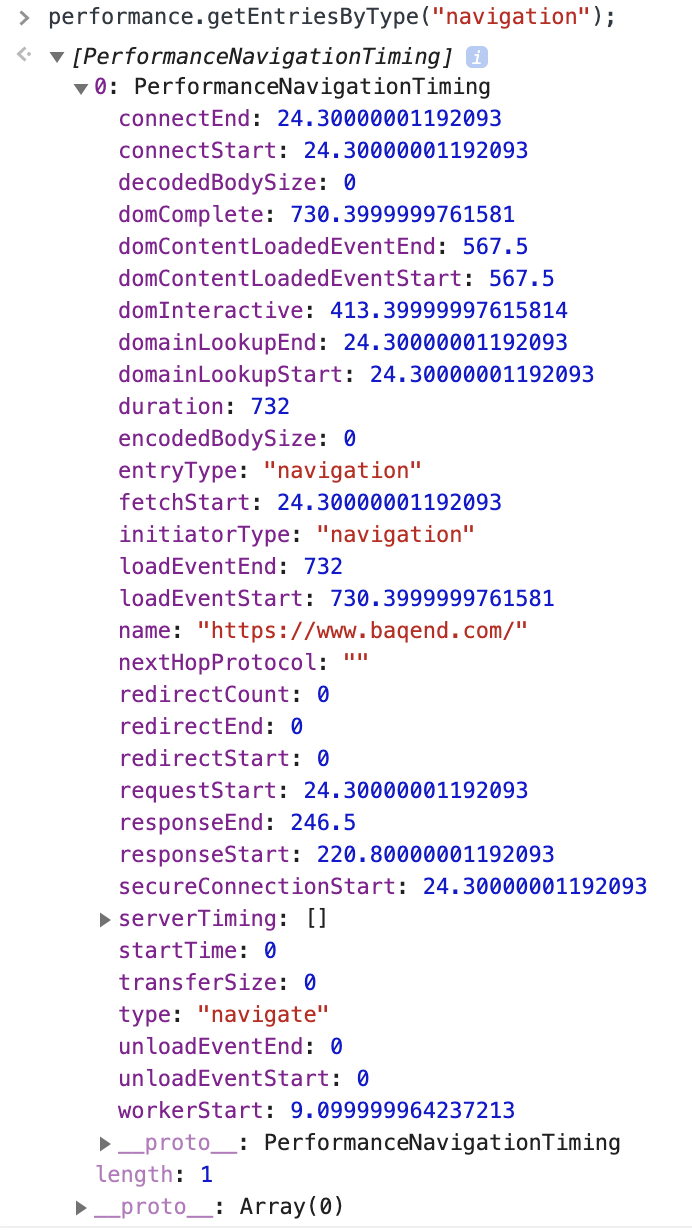
\includegraphics[width=0.4\textwidth]{navigation_console.png}
\caption{Navigation Timings}
\label{img:navigation_console}
\end{center}
\end{figure}


%TODO add this ?

% 2013 Grigorik
%- The real benefit of Navigation Timing is that it exposes a lot of previously inaccessible data, such as DNS and TCP connect times, with high precision (microsecond timestamps), via a standardized performance.timing object in each browser.
%- Hence, the data gathering process is very simple: load the page, grab the timing object from the user’s browser, and beacon it back to your analytics servers!
%- By capturing this data, we can observe real-world performance of our applications as seen by real users, on real hardware, and across a wide variety of different networks.

% 2013 Meenan
%- The largest benefit of navigation timing is that it exposes a lot of timings that lead up to the HTML loading --> This is this famous image
%- In addition to providing a good start time, it exposes information about any redirects, DNS lookup times, time to connect to the server, and how long it takes the Web server to respond to the request, for every user and for every page the user visits
%- The measurement points are exposed to the DOM (Document Object Model) through the performance object and make it trivial to calculate load times (or arbitrary intervals, really) from JavaScript.

% https://developer.mozilla.org/en-US/docs/Web/API/PerformanceNavigationTiming
%PerformanceNavigationTiming Interface: 
%- extends PerformanceEntry Interface from performance timeline. see attributes section for details
%- extends PerformanceResourceTiming Interface from resource timing


% ---------------------------------------------



\paragraph{Resource Timing}


% [Introduction]

Two versions of Resource Timing exist.
A Candidate Recommendation, Resource Timing Level 1, from March 2017, % https://www.w3.org/TR/resource-timing-1/
and Resource Timing Level 2, a Working Draft from April 2021.  % https://www.w3.org/TR/resource-timing-2/

As described above, while Navigation Timing exposes timing information for the main document, Resource Timing exposes timing information for all other resources the main document requests, and also resources other resources request.
Other resources may be CSS, JS, other HTML documents, images, and so on.
% https://www.w3.org/TR/resource-timing-2/

The exposed time stamps from Resource Timing are mainly network related timing values (see table X.)
For example, the time it takes to download a specific resource.


% [PerformanceResourceTiming Interface]

The values are exposed by the PerformanceResourceTiming interface and can be retrieved via $window.performance.getEntriesByType("resource")$.

% https://w3c.github.io/perf-timing-primer/
%- The PerformanceResourceTiming interface extends the PerformanceEntry interface in the Performance Timeline
%- Each of these timestamps is in microseconds, which are provided by the window.performance.now() method in the High Resolution Time specification.


% [Navigation and Resource Timing]

% https://www.w3.org/TR/resource-timing-2/
%- Navigation Timing 2 extends this specification to provide additional timing information associated with a navigation.
%- mechanisms to provide complete client-side latency measurements within applications

Navigation and Resource Timing go hand in hand.
With Navigation and Resource Timing, all relevant timing information for all resources of the website are available.
The Waterfall Chart (see section X.) is a picturesque example of a visualization of the exposed attributes by both specifications.

Figure X. depicts the values exposed by Navigation and Resource Timing.
Those attributes will be discussed next.




% ---------------------------------------------



\paragraph{Navigation and Resource Timing Attributes}

All timing values, or attributes, relevant for the navigation process and exposed by Navigation and Resource Timing Level 2, are listed in table X and figure X.
The black coloured time stamps assigned to the blue boxes in figure X. are captured by Navigation Timing.
The yellow time stamps are exposed by Resource Timing.
All attributes are retrievable via $performance.getEntriesByType("navigation")$.\footnote{They are exposed to navigation due to interface inheritance. For more details cf. } %cite navigation timing 2 spec
Figure X. does not include all defined and available values from the specification definitions, but only those important within the navigation process.
For documents from different origins, the attributes in parenthesis may not be available.% cite https://www.w3.org/TR/navigation-timing-2/#processing-model

\begin{figure}[h!]
\begin{center}
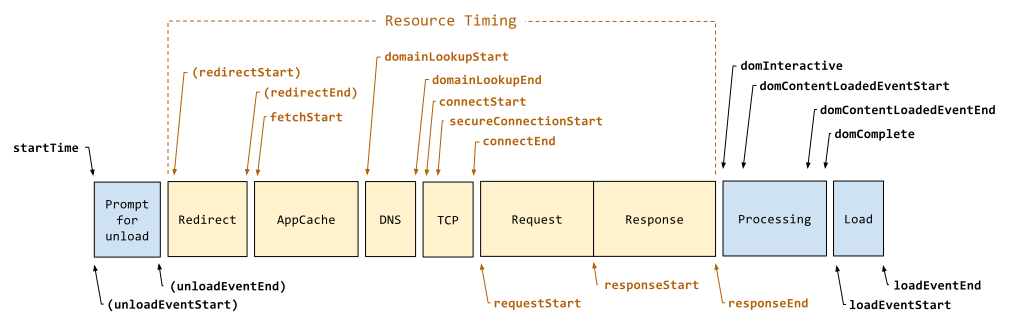
\includegraphics[width=1\textwidth]{timestamp_diagram.png}
\caption{Timestamps from Navigation and Resource Timing}
\label{img:latency}
\end{center}
\end{figure}
% cite https://www.w3.org/TR/navigation-timing-2/


Table X gives a short explanation for each time stamp.
The definitions are taken directly from the W3C specifications or MDN Web Docs, if not stated otherwise.
These time stamps are used to calculate performance metrics, as described in the next section.


%TODO is it ok to copy paste here from specs and MDN ?

\begin{center}
	\small
	\begin{longtable}{ | p{0.3\linewidth} | p{0.6\linewidth} | }
	\hline
	\multicolumn{2}{|c|}{ \cellcolor{lightgrey} Navigation Timings Level 2} \\
	\hline
	startTime (= navigationStart) & Start time of the navigation process. Is set to 0.  Navigation Timeline Level 1 exposes "navigationStart" which is set to the "time immediately after the user agent finishes prompting to unload the previous document."\footnote{\url{https://www.w3.org/TR/navigation-timing/)} [15.07.2021]} As many metrics calculations still rely on navigationStart as seen below, it is mentioned here. \\
	\hline
	unloadEventStart & Set to 0 if there is no previous document. Otherwise, value is set to time when previous documents unload event gets fired by the user agent. \\
	\hline
	unloadEventEnd & Set to 0 if there is no previous document.  .Otherwise, value is set to time when previous documents unload event ends. \\
	\hline
	domInteractive & Time value equal to the time immediately before the user agent sets the current document readiness of the current document to "interactive". \\
	\hline
	domContentLoadedEventStart & Time value equal to the time immediately before the user agent fires the DOMContentLoaded event at the current document. \\
	\hline
	domContentLoadedEventEnd & Time value equal to the time immediately after the current document's DOMContentLoaded event completes.  \\
	\hline
	domComplete & Time value equal to the time immediately before the user agent sets the current document readiness of the current document to "complete". \\
	\hline
	loadEventStart & Time value equal to the time immediately before the load event (window.onload ??) of the current document is fired.  Returns 0 if event has not been fired.  \\
	\hline
	loadEventEnd & Time value equal to the time when the load event of the current document is completed.  Returns 0 if event has not been fired or is not completed. \\

	\hline
	\multicolumn{2}{|c|}{ \cellcolor{lightgrey} Resource Timings Level 2} \\
	\hline
	redirectStart & Start time of the fetch which initiates the redirect. \\
	\hline
	redirectEnd & Marks timestamp which occurs immediately after receiving the last byte of the response of the last redirect. \\
	\hline
	fetchStart & Represents a timestamp immediately before the browser starts to fetch the resource. \\
	\hline
	domainLookupStart & Returns the timestamp immediately before the browser starts the domain name lookup for the resource. \\
	\hline
	domainLookupEnd & Returns the timestamp immediately after the browser finishes the domain name lookup for the resource. \\
	\hline
	connectStart & Returns the timestamp immediately before the user agent starts establishing the connection to the server to retrieve the resource. \\
	\hline
	connectEnd & Returns the timestamp immediately after the browser finishes establishing the connection to the server to retrieve the resource.  \\
	\hline
	secureConnectionStart & Returns a timestamp immediately before the browser starts the handshake process to secure the current connection.  \\
	\hline
	requestStart & Returns a timestamp of the time immediately before the browser starts requesting the resource from the server, cache, or local resource. \\
	\hline
	responseStart & Returns a timestamp immediately after the browser receives the first byte of the response from the server, cache, or local resource. \\
	\hline
	responseEnd & Returns a timestamp immediately after the browser receives the last byte of the resource or immediately before the transport connection is closed, whichever comes first. \\
	\hline
	\caption{Navigation and Resource Timing Level 2 Attributes} % needs to go inside longtable environment
	\label{tab:navigationtiming}
	\end{longtable}
\end{center}

%TODO check: is loadEventStart coming from window.onload or document.onload ?

%TODO add values from other interfaces such as duration ?
%from PerformanceEntry Interface:
%name
%entryType
%startTime
%duration

%TODO add exposed as DOMHighResTimeStamp ?


The document states and events mentioned above, such as DOMContentLoaded, and when they are fired by the user agent, are defined in the HTML standard.


%TODO add this when there is time...

% [Implementation Example Chrome]

% lets see how chromium is capturing domContentLoaded


% more infos here (probably level 1)
% https://community.akamai.com/customers/s/article/Using-Navigation-Timing-APIs-to-understand-your-webpage?language=en_US

% https://developers.google.com/web/fundamentals/performance/navigation-and-resource-timing
% Requests and responses:
%- fetchStart marks when the browser starts to fetch a resource. This is distinct from a request in that it doesn't mark when the browser makes a network request for a resource, but rather when it begins checking caches (e.g., HTTP and service worker caches) to see if a network request is even necessary.
%- workerStart marks when a request is being fetched from a service worker within a fetch event handler (if applicable). This will be always be 0 if a service worker isn't installed for the current page.



% ---------------------------------


\paragraph{Metrics calculated with Navigation and Resource Timing}

The attributes exposed by Navigation and Resource Timing are used to calculate common navigation timing metrics.
Table X. lists a selection of metrics and how they are being calculated.
Figure X. shows graphically which intervals the metrics are reflecting.


% Where are they coming from ?
% There are no official definitions of the metrics!

%Sometimes different vendors give a different name to the same metric.
%For many metrics there are no official definitions and the values diverge depending on the implementation.
%I will show how those metrics are being calculated.


\begin{figure}[h!]
\begin{center}
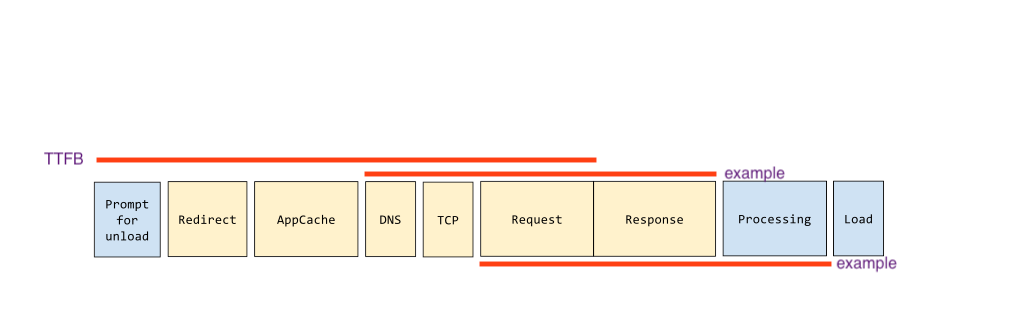
\includegraphics[width=1\textwidth]{timestamp_diagram_blank.png}
\caption{Navigation Timing Metrics}
\label{img:latency}
\end{center}
\end{figure}



% [Navigation Level 1 vs Level 2]

%- navigationStart is not in level 2
%- navigationStart is the same as startTime in level 2
%- Difference is that navigationStart is a EPOCH time stamp. The timings have to be calculated as differences to this timestamp
%- navigationStart just starts with 0, which makes all the other timestamps easier to read
%- many still use level 1 and navigationStart


%TODO add this ?

% [Calculations]
% Also maybe different calculations exist for the same metrc! check this again
% Basically i need to check how the different vendors / parties interpret the metric, e.g. how WPT calculates TTFB and GA



\begin{center}
	\small
	\begin{longtable}{ | p{0.3\linewidth} | p{0.6\linewidth} | }
	\hline
	Time to First Byte (TTFB) & $responseStart - navigationStart$: blablablabalb \\
	\hline
	Page Load Time (PLT) & $loadEventStart - navigationStart$ \\
	\hline
	DNS Lookup Time & $domainLookupEnd - domainLookupStart$ \\
	\hline
	TCP Handshake / Server Connect Time & $connectEnd - connectStart$ \\
	\hline
	TLS Handshake Time & $requestStart - secureConnectionStart$ \\
	\hline
	Request / Server Response Time & $responseStart - requestStart$ \\
	\hline
	DOM Content Loaded & $domContentLoadedEventEnd - domContentLoadedEventStart$ \\
	\hline
	Page Download Time & $responseEnd - responseStart$ \\
	\hline
	Latency & $responseStart - fetchStart$ \\
	\hline
	DOM Interactive & \\
	\hline
	DOM Complete & \\
	\hline
	Redirect & \\
	\hline
	\caption{Metrics} % needs to go inside longtable environment
	\label{tab:navigationtiming_metrics}
	\end{longtable}
\end{center}


% https://developer.mozilla.org/en-US/docs/Glossary




%TODO check out onload vs fully laoded vs page load time


% https://gtmetrix.com/blog/browser-timings/


% The loadEventStart attribute MUST return a DOMHighResTimeStamp with a time value equal to the time immediately before the load event of the current document is fired

% Onload 
% https://community.akamai.com/customers/s/article/Using-Navigation-Timing-APIs-to-understand-your-webpage?language=en_US

% https://developer.mozilla.org/en-US/docs/Web/API/GlobalEventHandlers/onload
% onload Event 
% Defined by the HTML specification


% https://www.stevesouders.com/blog/2013/05/13/moving-beyond-window-onload/


% https://speedcurve.com/blog/rendering-metrics/
%- In the old days, the main time-based performance metric was window.onload.




% TTFB

% https://developer.mozilla.org/en-US/docs/Glossary/time_to_first_byte
%TTFB = responseStart - navigationStart

% https://developer.mozilla.org/en-US/docs/Glossary/time_to_first_byte

% 2014 Hogan
%- First byte that the browser receives
%- It’s a good indicator of how quickly the backend of your site is able to process and send back content


% https://medium.baqend.com/mobile-site-speed-measurement-best-practices-ff4a3f91b003
%TTFB describes how long the requesting party has to wait from sending the first request packet until receiving the first response data packet





% PLT

% https://developer.mozilla.org/en-US/docs/Glossary/Page_load_time
%pageloadtime = time.loadEventStart - time.navigationStart;
% https://community.akamai.com/customers/s/article/Using-Navigation-Timing-APIs-to-understand-your-webpage?language=en_US

% 2013 Wang:
%- PLT as central metric

% 2018 Netravali

% https://hpbn.co/primer-on-web-performance/
%- Has been the de facto metric of the web performance world
%- Increasingly insufficient performance benchmark: we are no longer building pages, we are building dynamic and interactive web applications

% 2019 Enghardt







% Latency
% https://community.akamai.com/customers/s/article/Using-Navigation-Timing-APIs-to-understand-your-webpage?language=en_US
%responseStart – fetchStart




% DNS Lookup time
% https://developer.mozilla.org/en-US/docs/Web/Performance/Navigation_and_resource_timings#dns_lookup_time
%dns  = time.domainLookupEnd - time.domainLookupStart;
% https://developer.mozilla.org/en-US/docs/Web/Performance/Understanding_latency

% https://developers.google.com/web/fundamentals/performance/navigation-and-resource-timing
%domainLookupStart marks when a DNS lookup starts.
%domainLookupEnd marks when a DNS lookup ends.
%var pageNav = performance.getEntriesByType("navigation")[0];
%var dnsTime = pageNav.domainLookupEnd - pageNav.domainLookupStart;

%- both domainLookupStart and domainLookupEnd (and others) can be 0 for a resource served by a third party if that host doesn't set a proper Timing-Allow-Origin response heade

% https://community.akamai.com/customers/s/article/Using-Navigation-Timing-APIs-to-understand-your-webpage?language=en_US



% TCP / TCP Handshake Time / Server Connect Time
% https://developer.mozilla.org/en-US/docs/Web/Performance/Navigation_and_resource_timings#tcp
%tcp  = time.connectEnd - time.connectStart;

% https://community.akamai.com/customers/s/article/Using-Navigation-Timing-APIs-to-understand-your-webpage?language=en_US

% https://developer.mozilla.org/en-US/docs/Web/Performance/Understanding_latency



% TLS / SSL / TLS Handshake Time

% https://developer.mozilla.org/en-US/docs/Web/Performance/Navigation_and_resource_timings#ssl_negotiation
%ssl = time.requestStart - time.secureConnectionStart;

% https://developer.mozilla.org/en-US/docs/Web/Performance/Navigation_and_resource_timings#compression
%- compression savings percentage

% https://developers.google.com/web/fundamentals/performance/navigation-and-resource-timing
%- connection phase consists of three metrics
%- connectStart marks when the client opens a connection to the server.
%- secureConnectionStart marks when the client begins TLS negotiation.
%- connectEnd marks when connection negotiation ends (including TLS time).

%- var connectionTime = pageNav.connectEnd - pageNav.connectStart;
%- tlsTime = pageNav.connectEnd - pageNav.secureConnectionStart;


% https://developer.mozilla.org/en-US/docs/Web/Performance/Understanding_latency




% Request Time. / Server Response Time

% https://developer.mozilla.org/en-US/docs/Web/Performance/Navigation_and_resource_timings#request_time
%request = timing.responseStart - timing.requestStart

% https://community.akamai.com/customers/s/article/Using-Navigation-Timing-APIs-to-understand-your-webpage?language=en_US

% https://developer.mozilla.org/en-US/docs/Web/Performance/Understanding_latency






% Transfer/Page Download Time = responseEnd - responseStart

% https://community.akamai.com/customers/s/article/Using-Navigation-Timing-APIs-to-understand-your-webpage?language=en_US


% https://developer.mozilla.org/en-US/docs/Web/Performance/Understanding_latency
% Receiving / Download Time ??



% DOM Interactive Time
% https://community.akamai.com/customers/s/article/Using-Navigation-Timing-APIs-to-understand-your-webpage?language=en_US



% DOM Content Load Time

% https://community.akamai.com/customers/s/article/Using-Navigation-Timing-APIs-to-understand-your-webpage?language=en_US

% https://developer.mozilla.org/en-US/docs/Web/API/Window/DOMContentLoaded_event

% Defined by the HTML specification

% https://developer.mozilla.org/en-US/docs/Web/Performance/Navigation_and_resource_timings#domcontentloaded_event
% DOMContentLoaded = timing.domContentLoadedEventEnd - timing.domContentLoadedEventStart

% 2019 Enghardt




% DOM Processing to Interactive
% https://community.akamai.com/customers/s/article/Using-Navigation-Timing-APIs-to-understand-your-webpage?language=en_US


% DOM Interactive to Complete
% https://community.akamai.com/customers/s/article/Using-Navigation-Timing-APIs-to-understand-your-webpage?language=en_US


% Redirects
% https://developers.google.com/web/fundamentals/performance/navigation-and-resource-timing
% redirectStart and redirectEnd 






%TODO add this ?

%Load Event Duration
% https://developer.mozilla.org/en-US/docs/Web/Performance/Navigation_and_resource_timings#load_event_duration
%load = timing.loadEventEnd - timing.loadEventStart 


%Duration
% https://developer.mozilla.org/en-US/docs/Web/Performance/Navigation_and_resource_timings#duration
%duration = PerformanceNavigationTiming.loadEventEnd - PerformanceEntry.startTime
% -> duration from performanceentry interface is from loadEventStart - start Time



%Loading
% https://developers.google.com/web/fundamentals/performance/navigation-and-resource-timing
%- loadEventStart and loadEventEnd



%Document processing
% https://developers.google.com/web/fundamentals/performance/navigation-and-resource-timing
%- domInteractive, domContentLoadedEventStart, domContentLoadedEventEnd, and domComplete



%Unloading
% https://developers.google.com/web/fundamentals/performance/navigation-and-resource-timing
%Document unloading:
%- unloadEventStart and unloadEventEnd 


%Sizes
% https://developers.google.com/web/fundamentals/performance/navigation-and-resource-timing
%Document and resource size:
%- transferSize is the total size of the resource including HTTP headers.
%- encodedBodySize is the compressed size of the resource excluding HTTP headers.
%- decodedBodySize is the decompressed size of the resource (again, excluding HTTP headers).






% ------------------------------------------------
% ------------------------------------------------



Apart from Navigation and Resource Timing, the Web Performance Working Group also maintains other performance related specifications.
Some of them will be briefly discussed next.


\paragraph{User Timing}

User Timing Level 2 is a Recommendation from February 2019 and User Timing Level 3 is a Working Draft from July 2021.
User Timing provides methods to create own, specific and unique high resolution timestamps, to query them and to calculate intervals and the elapsed time between those created timestamps.% cite https://www.w3.org/TR/user-timing-3/
User Timing simplifies and facilitates the usage of custom metrics (see section X.)

% https://www.w3.org/TR/user-timing-3/
%- PerformanceMark and PerformanceMeasure interfaces

% Measuring Real User Performance in the Browser https://www.youtube.com/watch?v=yrWLi524YLM&ab_channel=NicJansma
%-> Puts data in Performance Timeline / DevTools


% -------------------


\paragraph{Performance Timeline}

Performance Timeline is a Recommendation from December 2013 % https://www.w3.org/TR/2013/REC-performance-timeline-20131212/
and Performance Timeline Level 2 is a Working Draft from June 2021. % https://www.w3.org/TR/performance-timeline-2/

In short, the Performance Timeline defines an API and methods which expose all timing values captured by other specifications such as Navigation or Resource Timing.
Performance Timeline defines an interface to acquire a variety of performance measurements. 
As already described, in can be used to retrieve Navigation Timings with $performance.getEntriesByType("navigation")$.

Additionally, a PerformanceObserver interface is defined, which can be used to monitor the Performance Timeline and notify as soon as new measurements and recordings are available.


%TODO add this ? is not so important...

% https://www.w3.org/TR/performance-timeline-2/
%- extends the High Resolution Time specification
%- providing methods to store and retrieve high resolution performance metric data.
%- Performance Timeline  defined by Navigation timing, resource timing, user timing and other interfaces
%- get Entries, by Type, by Name
%- Example entryType values defined by other specifications include: "mark" and "measure" [USER-TIMING-2], "navigation" [NAVIGATION-TIMING-2], "resource" [RESOURCE-TIMING-2], and "longtask"


% [Performance Entry]
	
% https://developer.mozilla.org/en-US/docs/Web/API/Performance_Timeline
%- PerformanceEntry interface encapsulates a single performance entry: a single data point or metric in the performance timeline


% https://developer.mozilla.org/en-US/docs/Web/API/PerformanceEntry
%- A performance entry can be directly created by making a performance mark or measure

%Always of type:
%- PerformanceMark
%- PerformanceMeasure
%- PerformanceFrameTiming
%- PerformanceNavigationTiming
%- PerformanceResourceTiming
%- PerformancePaintTiming

%Properties:
%- name
%- entryType
%- startTime
%- duration



% ----------------------------


\paragraph{Long Tasks}

Long Tasks API 1 has been released as a First Public Working Draft in September 2017.
The goal of the API is to detect "long tasks", this are tasks that occupy main thread for more than 50ms.
Long tasks are critical for performance as they block other critical tasks such as user input. % cite  https://www.w3.org/TR/longtasks-1/

% https://www.youtube.com/watch?v=6Ljq-Jn-EgU&ab_channel=GoogleChromeDevelopers
%- Long Tasks: Is it delightful? PerformanceObserver


% ----------------------------


\paragraph{Server Timing}

Server Timing is a Working Draft from June 2021.
With specifications such as Navigation and Resource Timing, the user agent has access to a variety of different timings regarding the navigation process.
Not visible nor available are measurement and timings within the server processing, e.g. database queries.
Server Timing addresses this problem by enabling a server to transfer and communicate performance related information to the user agent. % cite https://www.w3.org/TR/server-timing/



% ----------------------------


\paragraph{Paint Timing}

Paint Timing 1 has been released as a First Public Working Draft in September 2017.  
It specifies two "key moments" during the load process: First Paint (FP), and First Contentful Paint (FCP).
Table X. provides explanations for the key moments as they are defined in the specification. % cite https://www.w3.org/TR/paint-timing/

The metrics can be retrieved via $performance.getEntriesByType("paint")$.

\begin{center}
\small
	\begin{tabular}{ | p{0.3\linewidth} | p{0.6\linewidth} | }
	\hline
	First Paint & Marks the point when the browser renders anything that is visually different from what was on the screen prior to navigation \\ 
	\hline
	First Contentful Paint & The point when the browser renders the first bit of content from the DOM, which may be text, an image, SVG, or even a canvas element \\  
	\hline
	\end{tabular}
\end{center}


FP and FCP indicate when the user sees something different than the default white screen for the first time.
If the visual change is important or useful for the user is not reflected by FP or FCP. % cite 2013 Meenan



%TODO add more here ?

% https://developer.mozilla.org/en-US/docs/Glossary/First_paint
% https://developer.mozilla.org/en-US/docs/Glossary/First_contentful_paint

% A user centric metric pendant is Start Render.
% FP and FCP are visual metrics from a browsers perspective, and not from a users perspective, as they are derived from  and not the actual pixels on the screen.



% ------------------------------------------------------------------------------------------------------------------



\paragraph{Navigation Timing Metrics Conclusion}

We can measure time for different processes in the document loading process.
W3C defines specs for this.
Attributes exposed by those specs are used to calculate metrics.

Metrics are not defined officially and may diverge depending on implementation.

Table X provides an overview of all discussed specifications, in which maturity level they are available and why they are important.


%The W3C provides recommendations and drafts which expose interesting timing data in the browser. %leveraging
%The High Resolution Time recommendation enables exact, stable and reliable time measures.
%The Navigation and Resource Timing specifications expose all relevant time stamps on the document, or any resource respectively, loading process.
%The User Timing spec makes it possible for analysts and developers to mark and measure custom time stamps and expose them directly to the Performance Timeline.
%The Performance Timeline subsumes all exposed timing measures and is the go to place to fetch performance data.

%Or as Grigorik states it, "The combination of Navigation, Resource, and User timing APIs provides all the necessary tools to instrument and conduct real-user performance measurement for every web application" % cite 2013 Girgorik



\begin{center}
\small
	\begin{tabular}{ p{0.3\linewidth} | p{0.6\linewidth} }
	\hline
	High Resolution Time &
	\begin{itemize}[label={}, noitemsep,nolistsep, leftmargin=0cm]
		\item Level 2: REC November 2019
		\item WD July 2021
		\item Provides exact, stable and reliable time measures
	\end{itemize} \\
	\hline
	Navigation Timing &
	\begin{itemize}[label={}, noitemsep,nolistsep, leftmargin=0cm]
		\item Level 1: REC December 2021
		\item Level 2: WD March 2021
		\item Exposes navigation timing information of the main document
	\end{itemize} \\
	\hline
	Resource Timing &
	\begin{itemize}[label={}, noitemsep,nolistsep, leftmargin=0cm]
		\item Level 1: CR March 2017
		\item Level 2: WD April 2021
		\item Exposes timing information from requested resources and the resources they request. 
	\end{itemize} \\
	\hline
	Navigation and Resource Timing &
	\begin{itemize}[label={}, noitemsep,nolistsep, leftmargin=0cm]
		\item Used to calculated a variety of metrics
	\end{itemize} \\	
	\hline
	\hline
	User Timing & 
	\begin{itemize}[label={}, noitemsep,nolistsep, leftmargin=0cm]
		\item Level 2: REC February 2019
		\item Level 3: WD July 2021
		\item Mark and measure custom timestamps
	\end{itemize} \\  
	\hline
	Performance Timeline &
	\begin{itemize}[label={}, noitemsep,nolistsep, leftmargin=0cm]
		\item REC December 2013
		\item Level 2: WD June 2021
		\item Subsumes gathered performance data from other specifications
	\end{itemize} \\
	\hline
	Long Tasks &
	\begin{itemize}[label={}, noitemsep,nolistsep, leftmargin=0cm]
		\item API 1: FPWD  September 2017 
		\item Identify tasks occupying main thread for more than 50ms
	\end{itemize} \\	
	\hline
	Server Timing &
	\begin{itemize}[label={}, noitemsep,nolistsep, leftmargin=0cm]
		\item WD June 2021
		\item Standard to transmit performance related data from the server to the client
	\end{itemize} \\	
	\hline
	Paint Timing &
	\begin{itemize}[label={}, noitemsep,nolistsep, leftmargin=0cm]
		\item FPWD September 2017
	\end{itemize} \\
	\hline
	\end{tabular}
\end{center}


% [Transition]

%Multiple metrics are directly derived from those timing attributes, such as TTFB or Page Load Time.
%Those metrics cover only the technical aspect of performance, that is they reflect performance as time or how long it took for a specific task to finish.
%Those technical timing metrics may give an idea about the loading process of the web site, but they do not reflect how a user is experiencing the performance.

%The Paint Timing specification goes into the direction of capturing user perceived performance by exposing the time when the first visual content has been displayed to the user.

%This idea of user centric metrics has been followed by many such as Google, which introduces Web Vitals.
%Web Vitals are discussed in the next section, but before I will explain some other user centric metrics such as Speed Index.





% -----------------------------------------------------------------------
% -----------------------------------------------------------------------



\subsubsection{User-Centric Performance Metrics}


[tbd]


% [Introduction]

%Last section was about performance timings which are available through the web apis.
%They are timestamps and do not tell a lot about how the user perceives the performance.

% https://developer.mozilla.org/en-US/docs/Learn/Performance/Perceived_performance
%- Perceived performance
%- how fast a web site feels to a user
%- perception can be different that actual load times
%- more difficult to measure that loading times




%I will describe established user-centric performance metrics, such as TTI, TBT and Speed Index.
%Then I will discuss Web Vitals.



% ------------------------


\paragraph{Start Render}



% https://designingforperformance.com/basics-of-page-speed/
%- tells you how many seconds it took for the browser to begin rendering content


% https://blog.dareboost.com/en/2019/09/first-contentful-paint-fcp/


% 2018 Netravali
% TTFP


% 2019 Enghardt: TTFP





% ------------------------


\paragraph{Time to Interactive}

% https://developer.mozilla.org/en-US/docs/Glossary/Time_to_interactive



% 2018 Netravali
%- TTI


% https://www.youtube.com/watch?v=6Ljq-Jn-EgU&ab_channel=GoogleChromeDevelopers
%- Time To Interactive: Is it usable? Use Polyfill



% ------------------------


\paragraph{Total Blocking Time}

% https://web.dev/tbt/


% https://www.youtube.com/watch?v=6Ljq-Jn-EgU&ab_channel=GoogleChromeDevelopers
%- Total Blocking Time



% ------------------------



\paragraph{First Meaningful Paint}


% https://web.dev/first-meaningful-paint/
%- in seconds


%Replaced by LCP.

%how to measure lab and field


% https://www.youtube.com/watch?v=6Ljq-Jn-EgU&ab_channel=GoogleChromeDevelopers
%- First Meaningful Paint, Hero Element: Is it useful? 



% https://developer.mozilla.org/en-US/docs/Glossary/first_meaningful_paint

% https://medium.baqend.com/mobile-site-speed-measurement-best-practices-ff4a3f91b003
%The First Meaningful Paint is another user-centric metric and represents the point in time at which the largest visual change takes place; the underlying assumption here obviously is that the biggest visual change is relevant to the user, for example because a hero image or a navigation bar appear


% ------------------------


\paragraph{Above the Fold Time}


% 2013 Meenan

%- point in time when the last visual change is made to the visible part of the page
%- available only in lab environments where the visual progress of a page loading can be recorded


% 2018 Netravali
%- Above the fold time


% 2019 Enghardt


% ------------------------



\paragraph{Speed Index}


% https://docs.webpagetest.org/metrics/speedindex/


% https://developer.mozilla.org/en-US/docs/Glossary/Speed_index



% 2013 Meenan
%- best effort for representing the user experience in a single number


% 2018 Netravali


% 2021 Meenan vimeo 38:50



% Measuring Real User Performance in the Browser
%- How much of the screen is visually available at different points of time
%- At what point of time is the page complete


% https://medium.baqend.com/mobile-site-speed-measurement-best-practices-ff4a3f91b003
%The Speed Index revolves around visual completeness and represents the average time it takes for website elements to become visible. It works well for websites with a static layout, but is unreliable for websites with moving elements like carousels or videos. Computing the Speed Index for this kind of website requires a custom timer or event to demarcate the point in time at which visual completion is reached


% ------------------------



\paragraph{Web Vitals}


% [Introduction]


% https://web.dev/vitals/
%- "Web Vitals is an initiative by Google to provide unified guidance for quality signals that are essential to delivering a great user experience on the web."
%- Core Web Vitals: Metrics that matter the most
% - evolving: definitions and thresholds may change with greater frequency


% https://medium.baqend.com/mobile-site-speed-measurement-best-practices-ff4a3f91b003
%- a set of browser-based metrics for capturing user-perceived performance.
%- Google heralds the Web Vitals as the gold standard for website performance
%- publishes them in the Chrome User Experience Report (CrUX)



% [Types of Metrics]

% https://web.dev/user-centric-performance-metrics/
%- Perceived load speed
%- Load responsiveness
%- Runtime responsiveness
%- Visual stability
%- Smoothness



% [SEO]


% https://medium.baqend.com/mobile-site-speed-measurement-best-practices-ff4a3f91b003
%- The core metrics will further be used for ranking search results 
%- Website performance according to the Web Vitals will therefore be critically important for SEO in the upcoming years.



% [Key Questions]

 
\begin{center}
\small
	\begin{tabular}{ | p{0.3\linewidth} | p{0.6\linewidth} | }
	\hline
	\textit{Is it happening?} & 	Did the navigation start successfully? Has the server responded? \\
	\hline
	\textit{Is it useful?} & Has enough content rendered that users can engage with it? \\
	\hline
	\textit{Is it usable?} & Can users interact with the page, or is it busy? \\
	\hline
	\textit{Is it delightful?} & Are the interactions smooth and natural, free of lag and jank? \\
	\hline
	\end{tabular}
\end{center}
 % cite https://web.dev/user-centric-performance-metrics/





% [Core Web Vitals]


% https://web.dev/vitals/
%- apply to all web pages
%- available in all google tools
%- each core web vital  represents a distinct facet of the user experience: loading, interactivity, and visual stability
%- each is measurable in the field
%- rather stable in definition and thresholds
%- Collected by Crux, Pagespeed insights and search console
%- measure with library % https://github.com/GoogleChrome/web-vitals




% https://www.youtube.com/watch?v=iNfz9tg-wyg&ab_channel=GoogleChromeDevelopers
%- Future goals: Better support for Single Page Apps, Input responsiveness, Scrolling and animations
%- Areas of user experience beyond performance: Security, Privacy, Accessibility

 
%The core web vitals LCP CLS and FID are now being discussed. 


%TODO add this ?
% [Tools to measure]
% Osmani: Tools to measure
% Philip Walton. Best practices for measuring Web Vitals in the field


% ----------------------------------------



\paragraph{Largest Contentful Paint}



% LCP https://web.dev/lcp/


% https://www.youtube.com/watch?v=iNfz9tg-wyg&ab_channel=GoogleChromeDevelopers
%- LCP: Progressive loading.
%- FCP may become a core web vital



% https://wicg.github.io/largest-contentful-paint/



% https://medium.baqend.com/mobile-site-speed-measurement-best-practices-ff4a3f91b003
%- approximation of the First Meaningful Paint that can be captured in the browser




% [Measuring]
 
%- Google had some issues with capturing LCP in chrome, see twitter
%- Because of this they needed to release a new chrome version
%- CruX also has 2 different lcps now (?)
%- use this story to show that this stuff is far from trivial



% --------------------------


\paragraph{First Input Delay}

% FID https://web.dev/fid/


% https://www.youtube.com/watch?v=iNfz9tg-wyg&ab_channel=GoogleChromeDevelopers
%- FID: Interactivity during load


% [Measuring]



% --------------------------


\paragraph{Cumulative Layout Shift}

% CLS https://web.dev/cls/


% https://www.youtube.com/watch?v=iNfz9tg-wyg&ab_channel=GoogleChromeDevelopers
%- CLS: Visual stability


% [Measuring]


% New Measurement https://blog.webpagetest.org/posts/understanding-the-new-cumulative-layout-shift/?utm_medium=email&_hsmi=121601471&_hsenc=p2ANqtz-9IsSdXActEE6lw4BrDZNa4eFqzQZjgabLHbq7aS-c2KkhqLGNtkIaGfQYD4VqZe9_6ZYFlTmlCgB87THSfsnVM1fl7NiixtrJqAsVO6DPUjeJIo6c&utm_content=121601471&utm_source=hs_email


% --------------------------


\paragraph{Excursion: Thresholds and Benchmarks for Core Web Vitals}


[tbd]

% https://blog.chromium.org/2020/05/the-science-behind-web-vitals.html



% https://web.dev/defining-core-web-vitals-thresholds/



% [LCP]







% [FID]






% [CLS]









%TODO add this?
%- User perceived PLT




% -----------------------------------------------------------------------
% -----------------------------------------------------------------------



\subsubsection{Custom Metrics}


[tbd]

% 2013 Meenan
%- First, it is important to understand that no single number will answer that question. Even if you have defined exactly what you are trying to measure on your Web site, performance will vary widely across your user base and across the different pages on your site
%- Nothing beats application-specific knowledge and measurements

% 2021 Meenan
%- own / user specific metrics, e.g. time to first tweet for twitter 


% 2013 Grigork
%- "there is no one single metric that holds true for every application, which means that we must carefully define custom metrics in each case"
%-  "Custom and application-specific metrics are the key to establishing a sound performance strategy"


% https://web.dev/custom-metrics/
%- Universal metrics offer a good baseline, but in many cases you need to measure more than just these metrics in order to capture the full experience for your particular site.
%- Custom metrics allow you to measure aspects of your site's experience that may only apply to your site



% https://speedcurve.com/blog/user-timing-and-custom-metrics/



% -----------------------------------------------------------------------


\subsubsection{Metrics Conclusion}


[tbd]

%TODO ideally come up with a nice table which abstracts and summarizes everything about metrics:
% e.g. measured by: browser, server. Technical stuff is measured in browser, everything else not in browser
% technical, UX, ...

[summary table]



[Link to Research Question]


\paragraph{Observer Effect}

[tbd]

% https://www.youtube.com/watch?v=yrWLi524YLM&ab_channel=NicJansma
%Avoiding the Observer Effect

%- How to measure performance without affecting performance?
%- JS is single threaded
%- Unless browser is idle, anything you do in JS will slow down some other JS
%-> Do only cheap stuff
%- Don't slow down load time:
%	- Load measurement code outside the critical path
%	- Use Iframe Loader Technique
%	- Load measurement code after onload event (-> can not measure things that happen before onload)

%- Do as little as possible in event handlers
%- Do more expensive processing via requestIdleCallback that runs when browser is idle



% https://web.dev/custom-metrics/
%The first rule of effective performance measurement is to make sure your performance measurement techniques aren't causing performance issues themselves.



%Before tackling this question with an experiment, I will discuss one synthetic monitoring tool WPT and one RUM tool GA which I will then use in the approach.
%Also some research in this field will be discussed.




